\chapter{URG of Full Generalized SIAM}
\label{fullurg}
\section{The spin-charge-SIAM Hamiltonian}
In this section, we will consider the SIAM with both spin and charge fluctuations. This will be a combination of the last two sections. The total Hamiltonian will be
\begin{equation}\begin{aligned}
	\mathcal{H} =& \sum_{k\sigma}\tau_{k\sigma} + \epsilon_d \hat n_d + U \hat n_{d\uparrow}\hat n_{d \downarrow} + \sum_{k\sigma}\left( V_k c^\dagger_{k\sigma} c_{d\sigma} + \text{h.c.} \right) + J_z S_d^z\sum_{kk^\prime}\left( c^\dagger_{k \uparrow}c_{k^\prime \uparrow} - c^\dagger_{k \downarrow}c_{k^\prime \downarrow} \right) \\
	      &+ J_t \sum_{kk^\prime\sigma}c^\dagger_{d\sigma}c_{d\overline\sigma}c^\dagger_{k\overline\sigma}c_{k^\prime\sigma} + K_z C_d^z \sum_{kk^\prime}\left( c^\dagger_{k\sigma}c_{k^\prime\sigma} - \frac{1}{2}\delta_{kk^\prime} \right) + K_t \sum_{kk^\prime\sigma}\left(c^\dagger_{d\sigma}c^\dagger_{d\overline\sigma}c_{k\overline\sigma}c_{k^\prime\sigma}+\text{h.c.}\right)
\end{aligned}\end{equation}
\begin{figure}[!htb]
	\centering
	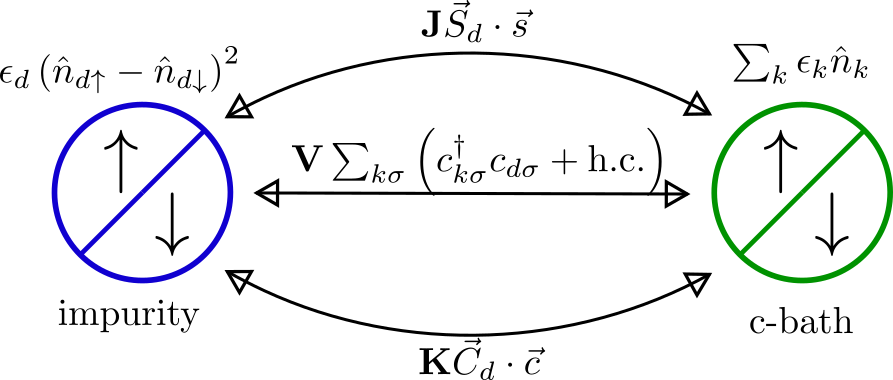
\includegraphics[width=0.5\textwidth]{../figures/gen_siam.png}
	\caption{Schematic diagram of the generalized SIAM model.}
\end{figure}
 There are eight different type of scattering terms:
\begin{equation}\begin{aligned}
	c^\dagger_{q\beta}T_1 &= V_1 c^\dagger_{q\beta}c_{d\beta}\hat n_{d\overline\beta}, &c^\dagger_{q\beta}T_2 &= V_0 c^\dagger_{q\beta}c_{d\beta}\left(1 - \hat n_{d\overline\beta}\right)\\
	c^\dagger_{q\beta}T_3 &= \sum_{k<\Lambda_N}J^z_0 \hat n_{d\beta}\left(1 - \hat n_{d\overline\beta}\right) c^\dagger_{q\beta}c_{k\beta}, &c^\dagger_{q\beta}T_4 &= -\sum_{k<\Lambda_N}J^z_1 \hat n_{d\overline\beta}\left(1 - \hat n_{d\beta}\right) c^\dagger_{q\beta}c_{k\beta}\\
	c^\dagger_{q\beta}T_5 &= \sum_{k<\Lambda_N}J^t c^\dagger_{d\overline\beta}c_{d\beta}c^\dagger_{q\beta}c_{k\overline\beta}, &c^\dagger_{q\beta}T_6 &= K_z^1 \sum_{k<\Lambda_N}\hat n_{d\beta}\hat n_{d\overline\beta}c^\dagger_{q\beta}c_{k\beta}\\
	c^\dagger_{q\beta}T_7 &= -K_z^0 \sum_{k<\Lambda_N}\left(1 - \hat n_{d\beta}\right)\left(1 - \hat n_{d\overline\beta}\right)c^\dagger_{q\beta}c_{k\beta}, &c^\dagger_{q\beta}T_8 &= K_t \sum_{k<\Lambda_N}c^\dagger_{q\beta}c^\dagger_{k\overline\beta}c_{d\overline\beta}c_{d\beta}\\
\end{aligned}\end{equation}

\section{Obtaining the RG equations}
\subsection{Particle Sector}
Renormalization is
\begin{equation}\begin{aligned}
	c^\dagger_{q\beta}T \eta = c^\dagger_{q\beta}\sum_{ij}T_i \eta_j
\end{aligned}\end{equation}
The terms that survive are
\begin{equation}\begin{aligned}
& c^\dagger_{q\beta}T \eta
= \sum_{i=1}^8\frac{1}{\omega_i - E_i}\hat n_{q\beta} T_i T_i^\dagger +\left(\frac{1}{\omega_2 - E_2} + \frac{1}{\omega_5 - E_5}\right)\hat n_{q\beta} \left(T_2 T_5^\dagger + T_5 T_2^\dagger \right) \\
& +\left(\frac{1}{\omega_2 - E_2} + \frac{1}{\omega_3 - E_3}\right)\hat n_{q\beta} \left(T_2 T_3^\dagger + T_3 T_2^\dagger \right) + \left(\frac{1}{\omega_3 - E_3} + \frac{1}{\omega_5 - E_5}\right)\hat n_{q\beta} \left(T_3 T_5^\dagger + T_5 T_3^\dagger \right) \\
& + \left(\frac{1}{\omega_1 - E_1} + \frac{1}{\omega_6 - E_6}\right)\hat n_{q\beta} \left(T_1 T_6^\dagger + T_6 T_1^\dagger \right) + \left(\frac{1}{\omega_1 - E_1} + \frac{1}{\omega_8 - E_8}\right)\hat n_{q\beta} \left(T_1 T_8^\dagger + T_8 T_1^\dagger \right) \\
& + \left(\frac{1}{\omega_6 - E_6} + \frac{1}{\omega_8 - E_8}\right)\hat n_{q\beta} \left(T_6 T_8^\dagger + T_8 T_6^\dagger \right)\\
&=\frac{|V_1|^2}{\xi_1}\left( 1 - \hat n_{d\beta} \right) \hat n_{d\overline\beta} + \frac{|V_0|^2}{\xi_2}\left( 1 - \hat n_{d\beta} \right) \left( 1 - \hat n_{d\overline\beta} \right) + \frac{1}{\xi_5}J_t^2 \left( 1 - \hat n_{d\beta} \right) \hat n_{d\overline\beta} c_{k^\prime\overline\beta}c^\dagger_{k\overline\beta} \\
&+ \frac{1}{4}\left[ {J_0^z}^2\frac{\hat n_{d\beta}\left( 1 - \hat n_{d\overline\beta} \right) }{\xi_3} + {J_1^z}^2\frac{\hat n_{d\overline\beta}\left( 1 - \hat n_{d\beta} \right)}{\xi_4} \right]c_{k^\prime\beta}c^\dagger_{k\beta} - \frac{1}{2} \left(\frac{1}{\xi_2} + \frac{1}{\xi_5}\right)J_t\left( 1 - \hat n_{d\beta}\right) \left(V_0 c^\dagger_{k\overline\beta}c_{d\overline\beta} + \text{h.c.}\right) \\
&- \frac{1}{2}\left(\frac{1}{\xi_2} + \frac{1}{\xi_3}\right)\frac{J^z_0}{2}\left(1 - \hat n_{d\overline\beta}\right)\left(V_0 c^\dagger_{k\beta}c_{d\beta} + \text{h.c.}\right) - \frac{1}{2}\left(\frac{1}{\xi_3} + \frac{1}{\xi_5}\right)\frac{J_t J^z_0}{2}\left(c^\dagger_{d\beta}c_{d\overline\beta}c^\dagger_{k\overline\beta}c_{k^\prime\beta} + \text{h.c.}\right) \\
&+ \left[\frac{{K_z^1}^2}{\xi_6}\hat n_{d\beta}\hat n_{d\overline\beta} + \frac{{K_z^0}^2}{\xi_7}\left(1 - \hat n_{d\beta}\right)\left(1 - \hat n_{d\overline\beta}\right)\right]c_{k^\prime\beta}c^\dagger_{k\beta} + \frac{K_t^2}{\xi_8}\left(1 - \hat n_{d\beta}\right)\left(1 - \hat n_{d\overline\beta}\right)c^\dagger_{k\overline\beta}c_{k^\prime\overline\beta}\\
&- \frac{1}{2}\left(\frac{1}{\xi_1} + \frac{1}{\xi_6} \right)V_1 K_z^1 \hat n_{d\overline\beta}\left(c^\dagger_{k\beta}c_{d\beta} + \text{h.c.}\right) + \frac{1}{2}\left(\frac{1}{\xi_1} + \frac{1}{\xi_8} \right)V_1 K_t \left(1 - \hat n_{d\beta}\right)\left(c^\dagger_{k\overline\beta}c_{d\overline\beta} + \text{h.c.}\right)\\
&- \frac{1}{2}\left(\frac{1}{\xi_6} + \frac{1}{\xi_8} \right)K_z^1 K_t \left(c^\dagger_{d\beta}c^\dagger_{d\overline\beta}c_{k^\prime\overline\beta}c_{k\beta} + \text{h.c.}\right)
\end{aligned}\end{equation}
where \(\xi_i = \omega_i - E_i\) and we substituted \(\hat n_{q\beta}=1\). The energies in the denominators are
\begin{equation}\begin{aligned}
E_1&= E_8 = \frac{\epsilon_q}{2} + 2\epsilon_d+ U - \frac{1}{2}K_z, &&E_2 = E_4 = E_5 = \frac{\epsilon_q}{2} + \epsilon_d - \frac{1}{2}J_z\\
E_3&=\frac{\epsilon_q}{2} + \epsilon_d + \frac{1}{2}J_z, &&E_6 =\frac{\epsilon_q}{2} + 2\epsilon_d+ U + \frac{1}{2}K_z\\
E_7&=\frac{\epsilon_q}{2} - \frac{1}{2}K_z, &&E_8=\frac{\epsilon_q}{2}+2\epsilon_d+ U  - \frac{1}{2}K_z
\end{aligned}\end{equation}
The quantum fluctuation scales are
\begin{equation}\begin{aligned}
\omega_1&=\omega + \epsilon_d+\frac{1}{2}K_z, &&\omega_3 =\omega+\epsilon_d + \frac{1}{2}K_z + J_z\\
\omega_2& = \omega_8 = \omega+\frac{1}{2}J_z, &&\omega_4 = \omega_5 = \omega + \epsilon_d + \frac{1}{2}K_z\\
\omega_6&=\omega+2\epsilon_d+U+\frac{1}{2}J_z + K_z, &&\omega_7 =\omega+\frac{1}{2}J_z\\
\end{aligned}\end{equation}
\subsection{Hole sector}
Renormalization is
\begin{equation}\begin{aligned}
&\eta c^\dagger_{q\beta}T = \left( 1 - \hat n_{q\beta} \right) \left[\sum_{i=1}^8\frac{1}{\omega^\prime_i - E^\prime_i} T_i T_i^\dagger +\left(\frac{1}{\omega^\prime_1 - E^\prime_1} + \frac{1}{\omega^\prime_4 - E^\prime_4}\right) \left(T_1 T_4^\dagger + T_4 T_1^\dagger \right)\right. \\
&\left. +\left(\frac{1}{\omega^\prime_1 - E^\prime_1} + \frac{1}{\omega^\prime_5 - E^\prime_5}\right) \left(T_1 T_5^\dagger + T_5 T_1^\dagger \right) + \left(\frac{1}{\omega^\prime_2 - E^\prime_2} + \frac{1}{\omega^\prime_7 - E^\prime_7}\right) \left(T_2 T_7^\dagger + T_7 T_2^\dagger \right) \right.\\
&\left. + \left(\frac{1}{\omega^\prime_2 - E^\prime_2} + \frac{2}{\omega^\prime_8 - E^\prime_8}\right) \left(T_2 T_8^\dagger + T_8 T_2^\dagger \right) + \left(\frac{1}{\omega^\prime_4 - E^\prime_4} + \frac{1}{\omega^\prime_5 - E^\prime_5}\right) \left(T_4 T_5^\dagger + T_5 T_4^\dagger \right) \right.\\
&\left. + \left(\frac{1}{\omega^\prime_7 - E^\prime_7} + \frac{1}{\omega^\prime_8 - E^\prime_8}\right)\hat n_{q\beta} \left(T_7 T_8^\dagger + T_8 T_7^\dagger \right)\right]\\
	&=\frac{|V_1|^2}{\xi^\prime_1}\hat n_{d\overline\beta}\hat n_{d\beta} + \frac{|V_0|^2}{\xi^\prime_2}\hat n_{d\beta}\left(1 - \hat n_{d\overline\beta}\right)+\frac{1}{4}\left[ {J_0^z}^2\frac{\hat n_{d\beta}\left( 1 - \hat n_{d\overline\beta} \right) }{\xi^\prime_3} + {J_1^z}^2\frac{\hat n_{d\overline\beta}\left( 1 - \hat n_{d\beta} \right)}{\xi^\prime_4} \right]c^\dagger_{k\beta}c_{k^\prime\beta} \\
	&+ \frac{1}{\xi^\prime_5}J_t^2 \left( 1 - \hat n_{d\overline\beta} \right) \hat n_{d\beta} c^\dagger_{k\overline\beta} c_{k^\prime\overline\beta} - \frac{1}{2} \left(\frac{1}{\xi^\prime_4} + \frac{1}{\xi^\prime_1}\right)\frac{J_1^z}{2}\hat n_{d\overline\beta} \left(V_1 c^\dagger_{k\beta}c_{d\beta} + \text{h.c.}\right) \\
	&- \frac{1}{2}\left(\frac{1}{\xi^\prime_1} + \frac{1}{\xi^\prime_5}\right)J_t \hat n_{d\beta}\left(V_1 c^\dagger_{k\overline\beta}c_{d\overline\beta} + \text{h.c.}\right) - \frac{1}{2}\left(\frac{1}{\xi^\prime_4} + \frac{1}{\xi^\prime_5}\right)\frac{J_t J^z_1}{2}\left(c^\dagger_{d\beta}c_{d\overline\beta}c^\dagger_{k\overline\beta}c_{k^\prime\beta} + \text{h.c.}\right)\\
&+\left[\frac{{K_z^1}^2}{\xi^\prime_6}\hat n_{d\beta}\hat n_{d\overline\beta} + \frac{{K_z^0}^2}{\xi^\prime_7}\left(1 - \hat n_{d\beta}\right)\left(1 - \hat n_{d\overline\beta}\right)\right]c^\dagger_{k\beta}c_{k^\prime\beta} + \frac{K_t^2}{\xi^\prime_8}\hat n_{d\beta}\hat n_{d\overline\beta}c_{k^\prime\overline\beta}c^\dagger_{k\overline\beta} \\
&- \frac{1}{2}\left(\frac{1}{\xi^\prime_2} + \frac{1}{\xi^\prime_7}\right)V_0 K_z^0\left(1 - \hat n_{d\overline\beta}\right)\left(c^\dagger_{k\beta}c_{d\beta} + \text{h.c.}\right) + \frac{1}{2}\left(\frac{1}{\xi^\prime_2} + \frac{1}{\xi^\prime_8}\right)V_0 K_t\hat n_{d\beta}\left(c^\dagger_{k\overline\beta}c_{d\overline\beta} + \text{h.c.}\right) \\
&- \frac{1}{2}\left(\frac{1}{\xi^\prime_7} + \frac{1}{\xi^\prime_8}\right)K_z^0 K_t\left(c^\dagger_{d\beta}c^\dagger_{d\overline\beta}c_{k\overline\beta}c_{k^\prime\beta} + \text{h.c.}\right) 
\end{aligned}\end{equation}
The denominator energies are
\begin{equation}\begin{aligned}
	E_1^\prime &= E_3^\prime = E_5^\prime = \frac{\epsilon_q}{2} + \epsilon_d - \frac{1}{2}J_z, &&E_4^\prime = \frac{\epsilon_q}{2} + \epsilon_d + \frac{1}{2}J_z\\
	E_2^\prime &= \frac{\epsilon_q}{2} - \frac{1}{2}K_z, &&E_7^\prime = \frac{\epsilon_q}{2} + \frac{1}{2}K_z\\
	E_6^\prime &= \frac{\epsilon_q}{2} + 2\epsilon_d + U - \frac{1}{2}K_z, &&E_8^\prime = \frac{\epsilon_q}{2} + \epsilon_d - \frac{1}{2}K_z\\
\end{aligned}\end{equation}
The quantum fluctuation scales are
\begin{equation}\begin{aligned}
	\omega_1^\prime&=\omega+2\epsilon_d+U+\frac{1}{2}J_z\\
	\omega_2^\prime&=\omega+\epsilon_d+\frac{1}{2}K_z \\
	\omega_3^\prime&=\omega_5^\prime=\omega+\epsilon_d + \frac{1}{2}K_z\\
	\omega_4^\prime&=\omega+\epsilon_d+\frac{1}{2}K_z + J_z \\
	\omega_6^\prime&=\omega+2\epsilon_d+U+\frac{1}{2}J_z\\
	\omega_7^\prime&=\omega+\frac{1}{2}J_z + K_z\\
	\omega_8^\prime &=\omega+\epsilon_d+\frac{1}{2}J_z \\
\end{aligned}\end{equation}
\subsection{Scaling equations}
The denominators \(\xi_i,\xi_i^\prime\) are
\begin{equation}\begin{aligned}
	\xi_1 &= \omega - \frac{\epsilon_q}{2} - \epsilon_d - U + K_z\\
	\xi_2 &= \omega - \frac{\epsilon_q}{2} - \epsilon_d + J_z\\
	\xi_3 &= \xi_4 = \xi_5 = \xi_6 = \xi_7 = \omega - \frac{\epsilon_q}{2} + \frac{1}{2}J_z + \frac{1}{2}K_z\\
	\xi_8 &= \omega - \frac{\epsilon_q}{2} - 2\epsilon_d - U + \frac{1}{2}J_z + \frac{1}{2}K_z\\
	\xi_1^\prime &= \omega - \frac{\epsilon_q}{2} + \epsilon_d + U + J_z\\
	\xi_2^\prime &= \omega - \frac{\epsilon_q}{2} + \epsilon_d + K_z\\
	\xi_3^\prime &= \xi_4^\prime = \xi_5^\prime = \xi_6^\prime = \xi_7^\prime = \omega - \frac{\epsilon_q}{2} + \frac{1}{2}J_z + \frac{1}{2}K_z\\
	\xi_8^\prime &= \omega - \frac{\epsilon_q}{2} + 2\epsilon_d + U + \frac{1}{2}J_z + \frac{1}{2}K_z\\
\end{aligned}\end{equation}
The RG equations are
\begin{equation}\begin{aligned}
	\Delta \epsilon_d &= \frac{|V_1|^2}{\xi_1} + \frac{|V_0|^2}{\xi_2^\prime} - 2 \frac{|V_0|^2}{\xi_2} - \sum_k\left( \frac{K_z^2}{2\xi_6} + \frac{K_t^2}{\xi_8} - \frac{J_z^2}{2\xi_3} - \frac{J_t^2}{\xi_3}\right) \\
	\Delta U &= \frac{2|V_1|^2}{\xi^\prime_1} + \frac{2|V_0|^2}{\xi_2} - \frac{2|V_1|^2}{\xi_1} - \frac{2|V_0|^2}{\xi_2^\prime} + 2\sum_k\left(\frac{K_z^2}{2\xi_6} + \frac{K_t^2}{\xi_8} - \frac{J_z^2}{2\xi_3} - \frac{J_t^2}{\xi_3}\right) \\
	\Delta V_1 &= - \frac{1}{4}\left[ V_1 \frac{K_z}{2}\left( \frac{1}{\xi_1} + \frac{1}{\xi_6} \right) - V_0 K_t \left( \frac{1}{\xi_2^\prime} + \frac{1}{\xi_8^\prime} \right)\right] - V_1 \left( \frac{J_z}{2} + J_t \right) \left( \frac{1}{\xi_1^\prime} + \frac{1}{\xi_3} \right) \\
	\Delta V_0 &= - \frac{1}{4}\left[ V_0 \frac{K_z}{2}\left( \frac{1}{\xi_2^\prime} + \frac{1}{\xi_7^\prime} \right) - V_1 K_t \left( \frac{1}{\xi_1} + \frac{1}{\xi_8} \right)\right] - V_0 \left( \frac{J_z}{2} + J_t \right) \left( \frac{1}{\xi_2} + \frac{1}{\xi_3} \right) \\
	\Delta J_z &= - 2 \frac{J_t^2}{\xi_3}\\
	\Delta J_t &= - 2 \frac{J_z J_t}{\xi_3}\\
	\Delta K_z &= - 2 \frac{K_t^2}{\xi_8}\\
	\Delta K_t &= - \frac{K_z K_t}{2}\left( \frac{1}{\xi_6} + \frac{1}{\xi_8} + \frac{1}{\xi_7^\prime} + \frac{1}{\xi_8^\prime}\right) \\
\end{aligned}\end{equation}
Note that these are the renormalizations are for each momentum state \(q\) on the isoenergetic shell - the total renormalization is obtained by summing over the \(q\).
\section{Numerical and analytical analysis of the symmetric model}
\subsection{Nature of RG flows for the symmetric model at \(V = 0\)}
With the conditions \(\epsilon_d = -\epsilon_d - U, J_z = J_t = \frac{1}{2}J, V_0 = V_1, K_z = K_t = \frac{1}{2}K\),
\begin{equation}\begin{aligned}
	\Delta U &= \sum_k \frac{3}{4}\frac{K^2 - J^2}{\omega - \frac{\epsilon_q}{2} + \frac{1}{4}J + \frac{1}{4}K} \\
	\Delta J &= - \frac{J^2}{\omega - \frac{\epsilon_q}{2} + \frac{1}{4}J + \frac{1}{4}K}\\
	\Delta K &= - \frac{K^2}{\omega - \frac{\epsilon_q}{2} + \frac{1}{4}J + \frac{1}{4}K}\\
\end{aligned}\end{equation}
For \(\omega - \frac{\epsilon_q}{2} + \frac{1}{4}J + \frac{1}{4}K > 0\), the flow is towards a weak coupling theory, but these are not URG fixed points. Such flows are shown in fig.~\ref{Jdecay}. For the rest of the values of \(\omega\), we get RG flows towards a strong-coupling fixed point, with large value of \(J\) and \(K\), fig.~\ref{J_sc}. For sufficiently small values of \(\frac{J}{K}\), the flow is towards zero \(U\). All such flows characterise a resonant-level strong coupling fixed point, where the four atomic impurity levels are degenerate and located exactly at the Fermi surface. For larger values of \(\frac{J}{K}\), there exist flows towards a large positive \(U\). Such fixed points energetically favour an impurity occupation of \(1\). Both these classes of flows of \(U\) are depicted in fig.~\ref{U_flow}.
\begin{figure}[!htb]
	\centering
	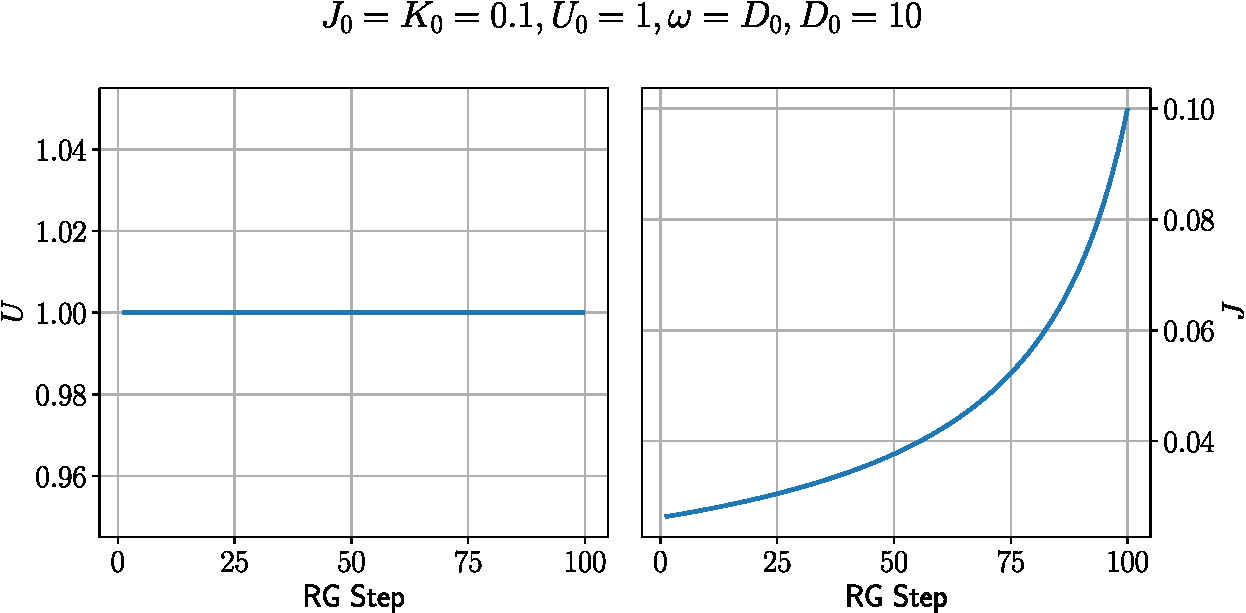
\includegraphics[width=\textwidth]{../figures/large_w.pdf}
	\caption{Large \(\omega\). Right Decay of \(J\) towards zero under RG. Left Flow of \(U\) under the same RG. Titles of plots show bare values.}
	\label{Jdecay}
\end{figure}
\begin{figure}[htb!]
	\centering
	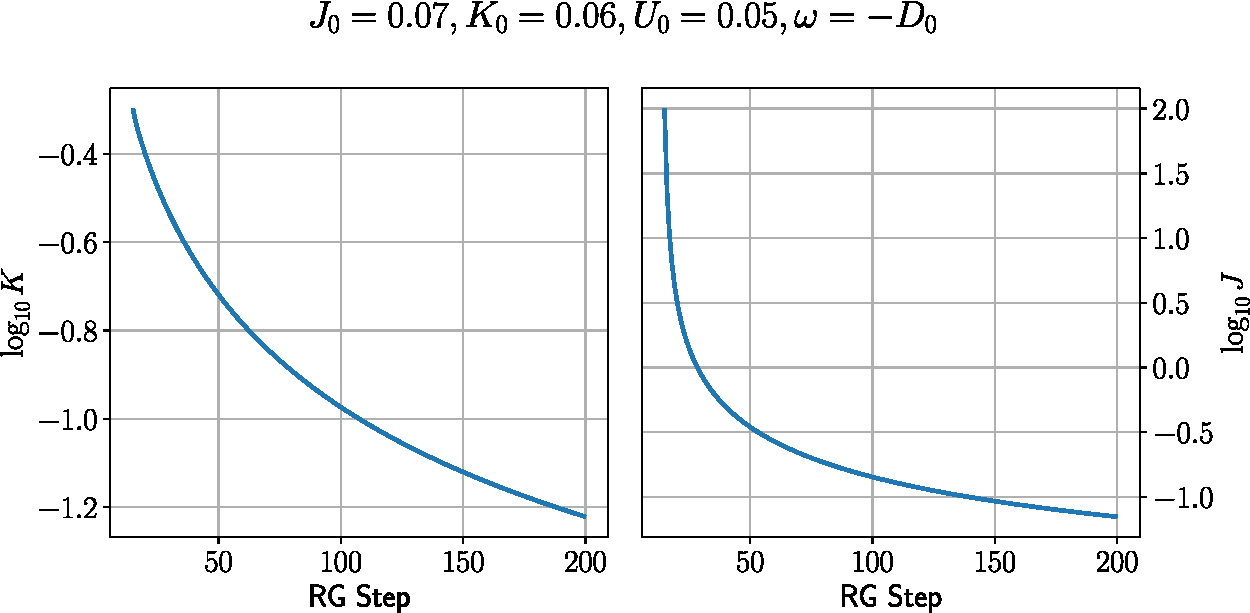
\includegraphics[width=\textwidth]{../figures/low_w_JK.pdf}
	\caption{Small \(\omega\). Flow of \(J\) and \(K\) to large values, signaling a strong-coupling fixed point.}
	\label{J_sc}
\end{figure}
\begin{figure}[!htb]
	\centering
	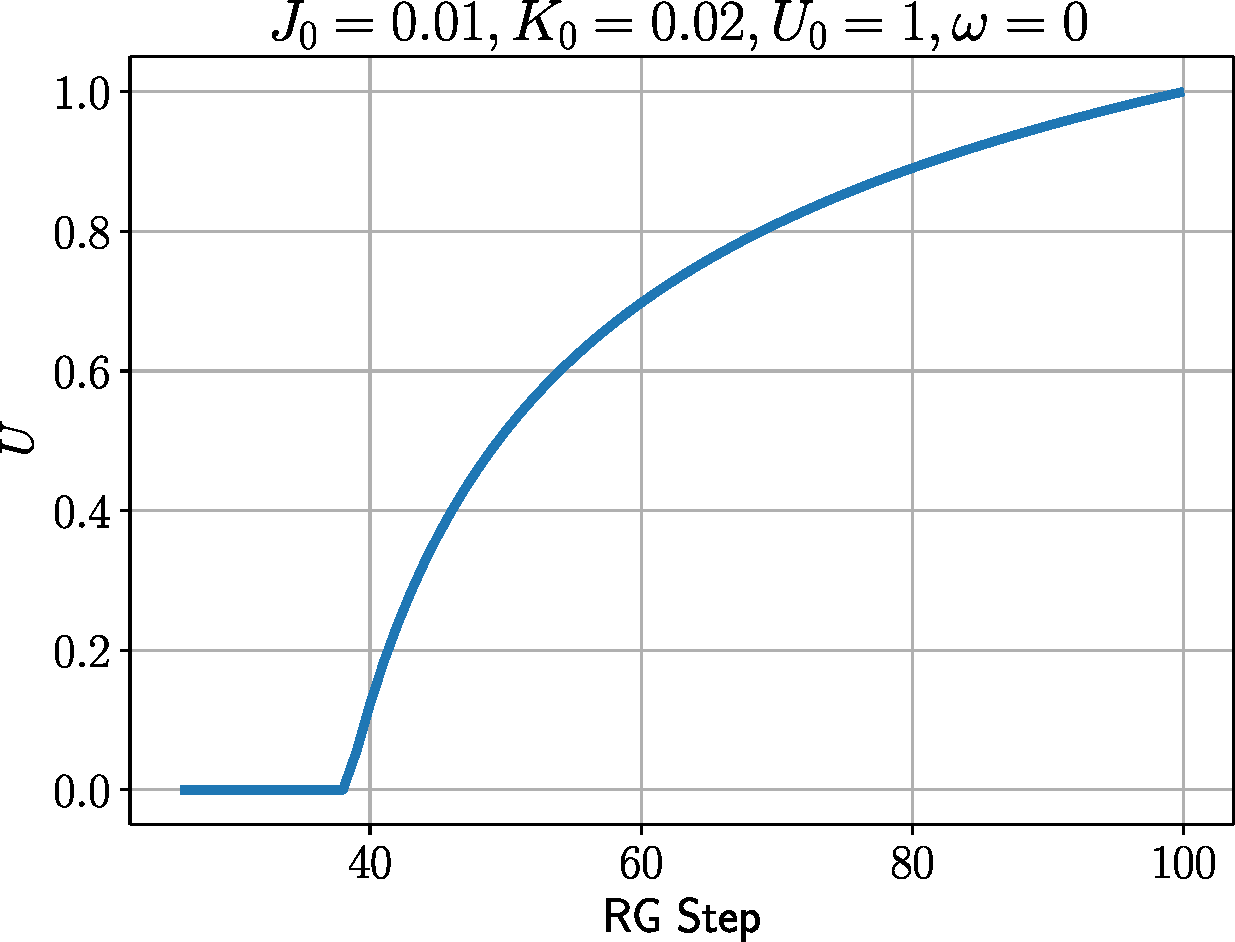
\includegraphics[width=0.49\textwidth]{../figures/U_irr.pdf}
	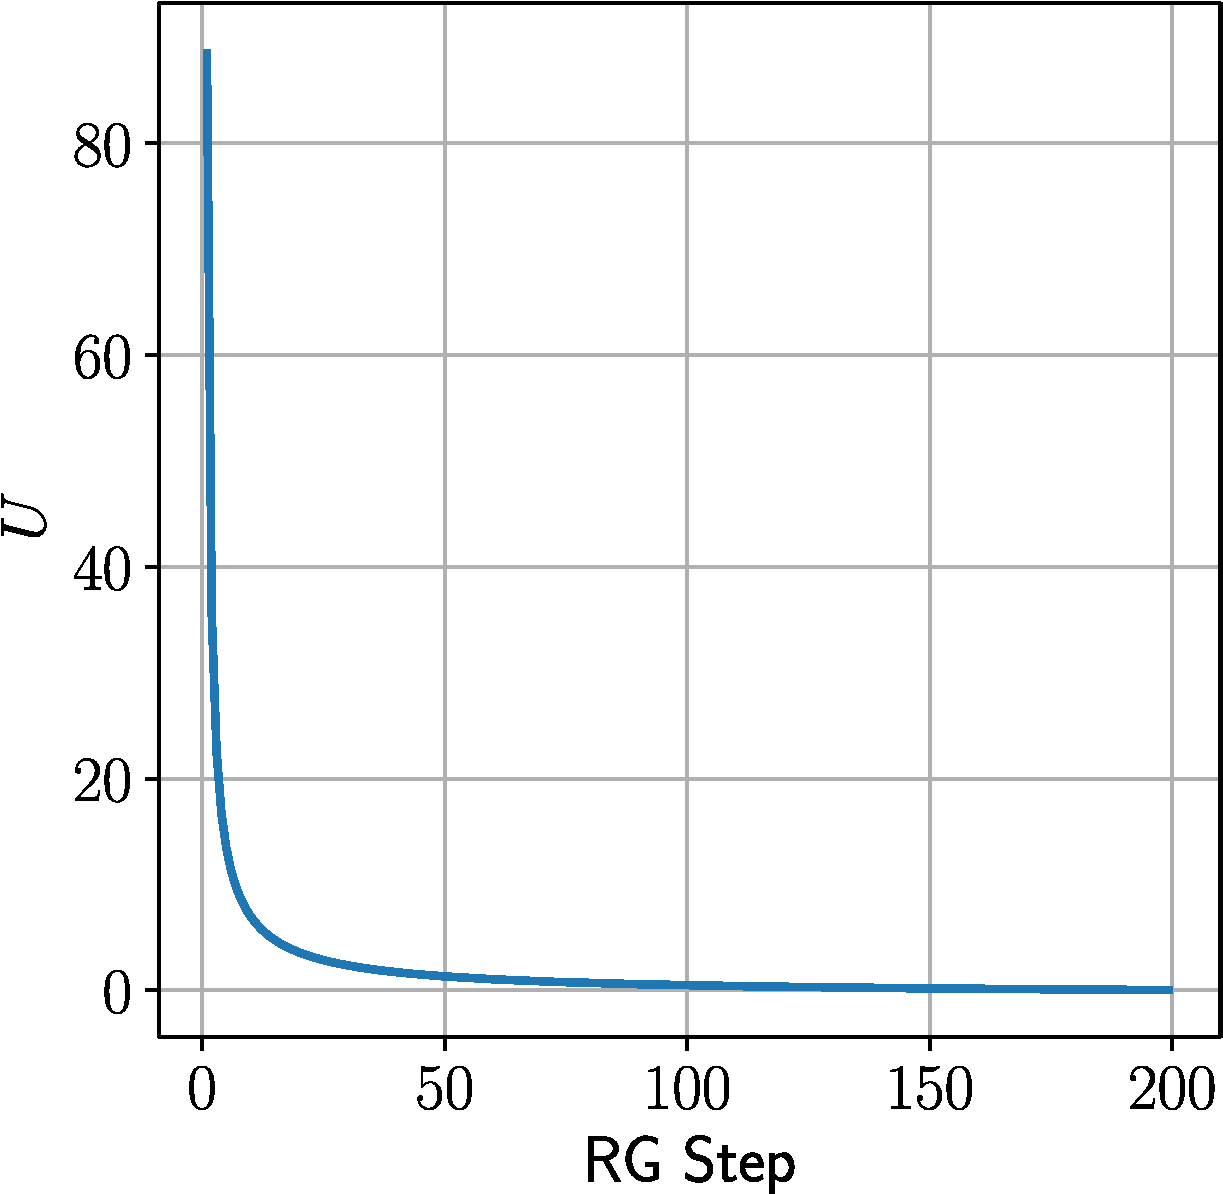
\includegraphics[width=0.49\textwidth]{../figures/U_rel.pdf}
	\caption{Left: Flow of \(U\) to zero, implying a four-fold degenerate impurity. Right: Flow of \(U\) to large value, making the impurity singly-occupied, leading to the formation of a local moment.}
	\label{U_flow}
\end{figure}
From the RG equations for \(J\) and \(K\), we can write down an RG-invariant.
\begin{equation}\begin{aligned}
	\label{rginv}
	\frac{\Delta J}{\Delta K} = \frac{J^2}{K^2} \implies \frac{1}{J} - \frac{1}{K} = \mathcal{C} = \frac{1}{J_0} - \frac{1}{K_0}
\end{aligned}\end{equation}
where \(\mathcal{C}\) is a constant. For the case of \(J_0 = K_0\) (\(J_0\) is the bare value of \(J\)), we must have \(J=K\). The RG flows in the \(K \text{ vs } J\) plane are shown in fig.~\ref{JvsK}.
\begin{figure}[!htb]
	\centering
	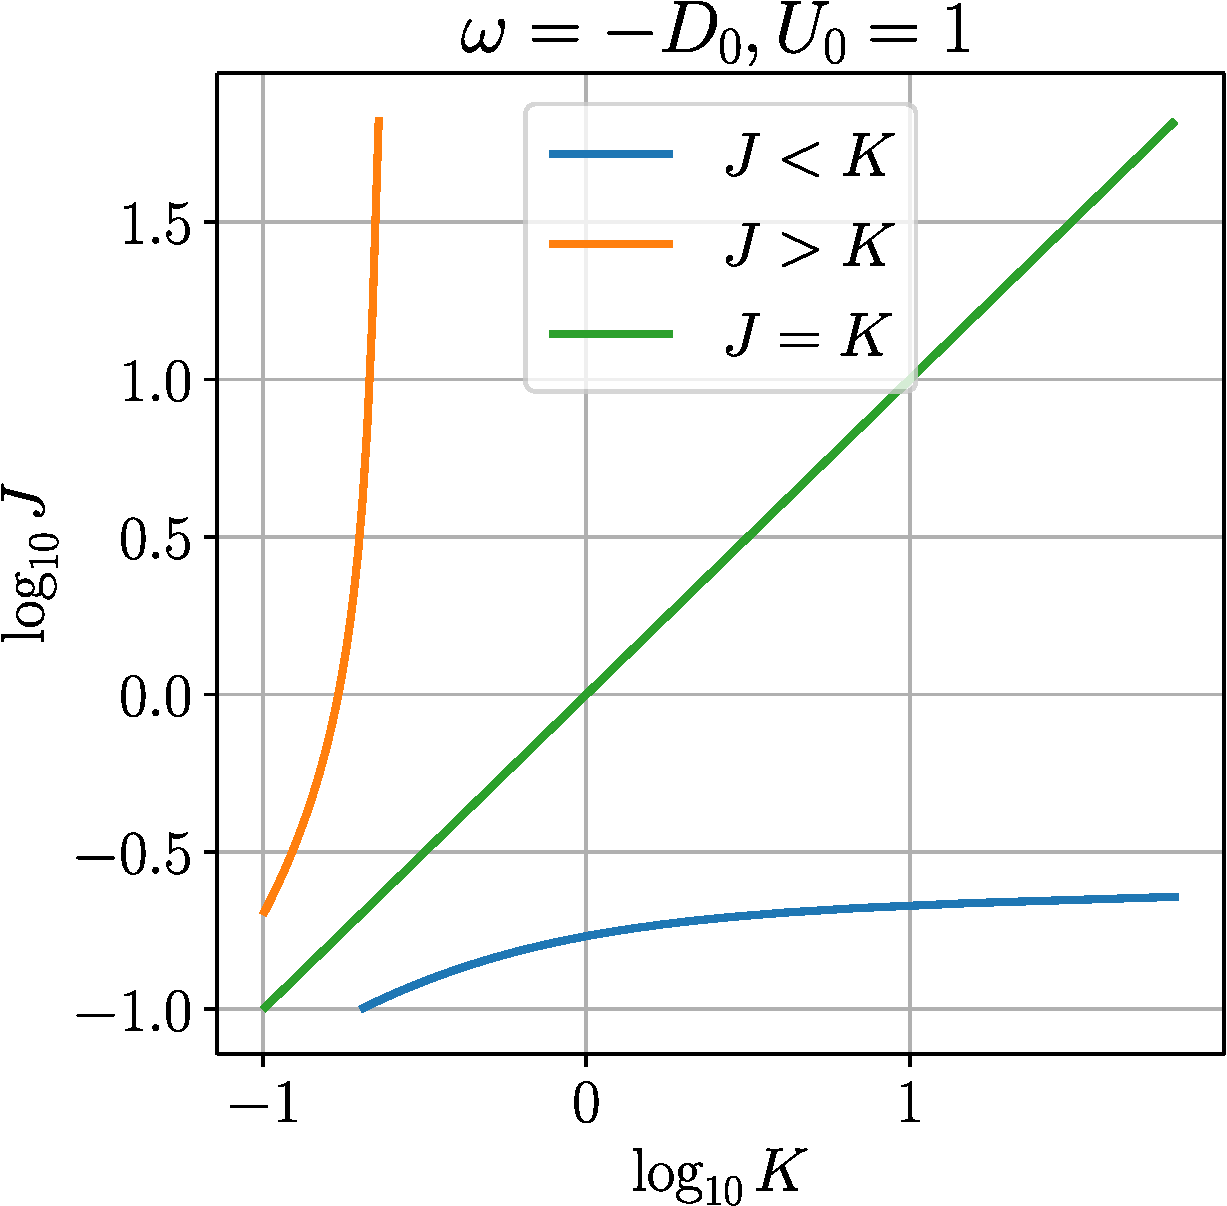
\includegraphics[width=0.6\textwidth]{../figures/JvsK.pdf}
	\caption{RG flows in \(K\) vs \(J\) plane. Legend indicates relations of bare values.}
	\label{JvsK}
\end{figure}
\subsection{Eigenstates of symmetrical model at \(V=0\)}
For the case of \(V=0\), the RG equations simplify considerably.
\begin{equation}\begin{aligned}
	\Delta U &= 2\sum_k \frac{3}{8}\frac{K^2 - J^2}{\omega - \frac{\epsilon_q}{2} + \frac{1}{4}J + \frac{1}{4}K} \\
	\Delta J &= - \frac{J^2}{\omega - \frac{\epsilon_q}{2} + \frac{1}{4}J + \frac{1}{4}K}\\
	\Delta K &= - \frac{K^2}{\omega - \frac{\epsilon_q}{2} + \frac{1}{4}J + \frac{1}{4}K}\\
\end{aligned}\end{equation}
The strong-coupling fixed points is reached for \(\omega - \frac{\epsilon_q}{2} + \frac{1}{4}J + \frac{1}{4}K < 0\). Since the denominator is thus negative, we will have
\begin{equation}\begin{aligned}
	\Delta U \begin{cases}
		> 0, & J> K \\
		< 0, & J< K
	\end{cases}
\end{aligned}\end{equation}
This implies that for \(J>K\), the flow is towards an impurity which is singly-occupied, while \(J < K\) will mean the impurity will be four-fold degenerate with all four levels at the Fermi surface. 

The effective Hamiltonian is
\begin{equation}\begin{aligned}
	\mathcal{H}^* = \sum_{k\sigma} \epsilon_k \hat n_{k\sigma} - 2 U^* \left(S_d^z\right)^2 + \sum_{kk^\prime < \Lambda^*}\left[J^* \vec{S_d}\cdot\vec{s_{kk^\prime}} + K^* \vec{C_d}\cdot\vec{C_{kk^\prime}}\right] + \sum_{q > \Lambda^*}\left[J_q S_d^z s^z_{q} + K_q C_d^z C^z_{q}\right]
\end{aligned}\end{equation}
where \(S_d^z = \frac{1}{2}\left( \hat n_{d\uparrow} - \hat n_{d \downarrow} \right) \). Since the interaction terms do not couple the \(\hat n_{d}=1\) and \(\hat n_{d}=0,2\) subspaces, we can diagonalize the Hamiltonian separately in these subspaces. 

In the singly-occupied subspace, the Hamiltonian is
\begin{equation}\begin{aligned}
	\mathcal{H}^*_{1} = \sum_k \epsilon_k \hat n_{k\sigma} - \frac{1}{2} U^* + \sum_{kk^\prime < \Lambda^*}J^* \vec{S_d}\cdot\vec{s_{kk^\prime}}+ \sum_{q > \Lambda^*}J^{**} S_d^z s^z_{q}
\end{aligned}\end{equation}
The ground state in this subspace is
\begin{equation}\begin{aligned}
	\ket{\Psi}^*_{1}= \frac{1}{\mathcal{N}}\sum_{kk^\prime < \Lambda^*\atop{q>\Lambda^*}}\left[\ket{S_d^z= \frac{1}{2}}\ket{s^z_{kk^\prime}= - \frac{1}{2}}\ket{s^z_{q}= - \frac{1}{2}} - \ket{S_d^z=- \frac{1}{2}}\ket{s^z_{kk^\prime}=  \frac{1}{2}}\ket{s^z_{q}=  \frac{1}{2}}\right]
\end{aligned}\end{equation}
with an eigenvalue (besides the energy of the bath)
\begin{equation}\begin{aligned}
	E_{1} = - \frac{U^*}{2} - \frac{3}{4}J^* - \frac{1}{4}J^{**}
\end{aligned}\end{equation}
In the complementary subspace, the Hamiltonian is
\begin{equation}\begin{aligned}
	\mathcal{H}^*_{0,2} = \sum_k \epsilon_k \hat n_{k\sigma} + \sum_{kk^\prime < \Lambda^*}K^* \vec{C_d}\cdot\vec{C_{kk^\prime}}+ \sum_{q > \Lambda^*}K^{**} C_d^z C^z_{q}
\end{aligned}\end{equation}
The ground state in this subspace is
\begin{equation}\begin{aligned}
	\ket{\Psi}^*_{0,2}= \frac{1}{\mathcal{N^\prime}}\sum_{kk^\prime < \Lambda^*\atop{q>\Lambda^*}}\left[\ket{C_d^z= \frac{1}{2}}\ket{C^z_{kk^\prime}= - \frac{1}{2}}\ket{C^z_{q}= - \frac{1}{2}} - \ket{C_d^z=- \frac{1}{2}}\ket{C^z_{kk^\prime}=  \frac{1}{2}}\ket{C^z_{q}=  \frac{1}{2}}\right]
\end{aligned}\end{equation}
with an eigenvalue (besides the energy of the bath)
\begin{equation}\begin{aligned}
	E_{0,2} = - \frac{3}{4}K^* - \frac{1}{4}K^{**}
\end{aligned}\end{equation}
Depending on the bare values of \(J,K\) and \(U\), we can have the following fixed point situations:
\begin{table}[!htb]
\centering
\begin{tabular}{|c|c|c|c|c|c|c|}
\hline
\(U \) & \(J,K \) & \(U^*\) &\(J^*,K^*\) & class & ground state & ground state energy\\
\hline
\(>0\)& \(J > K\)& \(\gg 0\)&\(J^*>K^*\) & screened spin & spin singlet & \(- \frac{U^*}{2} - \frac{3}{4}J^* - \frac{1}{4}J^{**}\)\\
\(>0\)& \(J < K\)& \(0\) &\(J^*<K^*\) & screened charge & charge singlet & \(- \frac{3}{4}K^* - \frac{1}{4}K^{**}\)\\
\(<0\)& \(J > K\)& \(0\) &\(J^*>K^*\) & screened spin & spin singlet& \(- \frac{3}{4}J^* - \frac{1}{4}J^{**}\)\\
\(<0\)& \(J < K\)& \(\ll 0\)&\(J^*<K^*\) & screened charge & charge singlet & \(- \frac{3}{4}K^* - \frac{1}{4}K^{**}\)\\
\hline
\end{tabular}
\caption{Classification of fixed points for various bare values, at \(V=0\)}
\label{classes}
\end{table}
\begin{figure}[htb!]
	\centering
	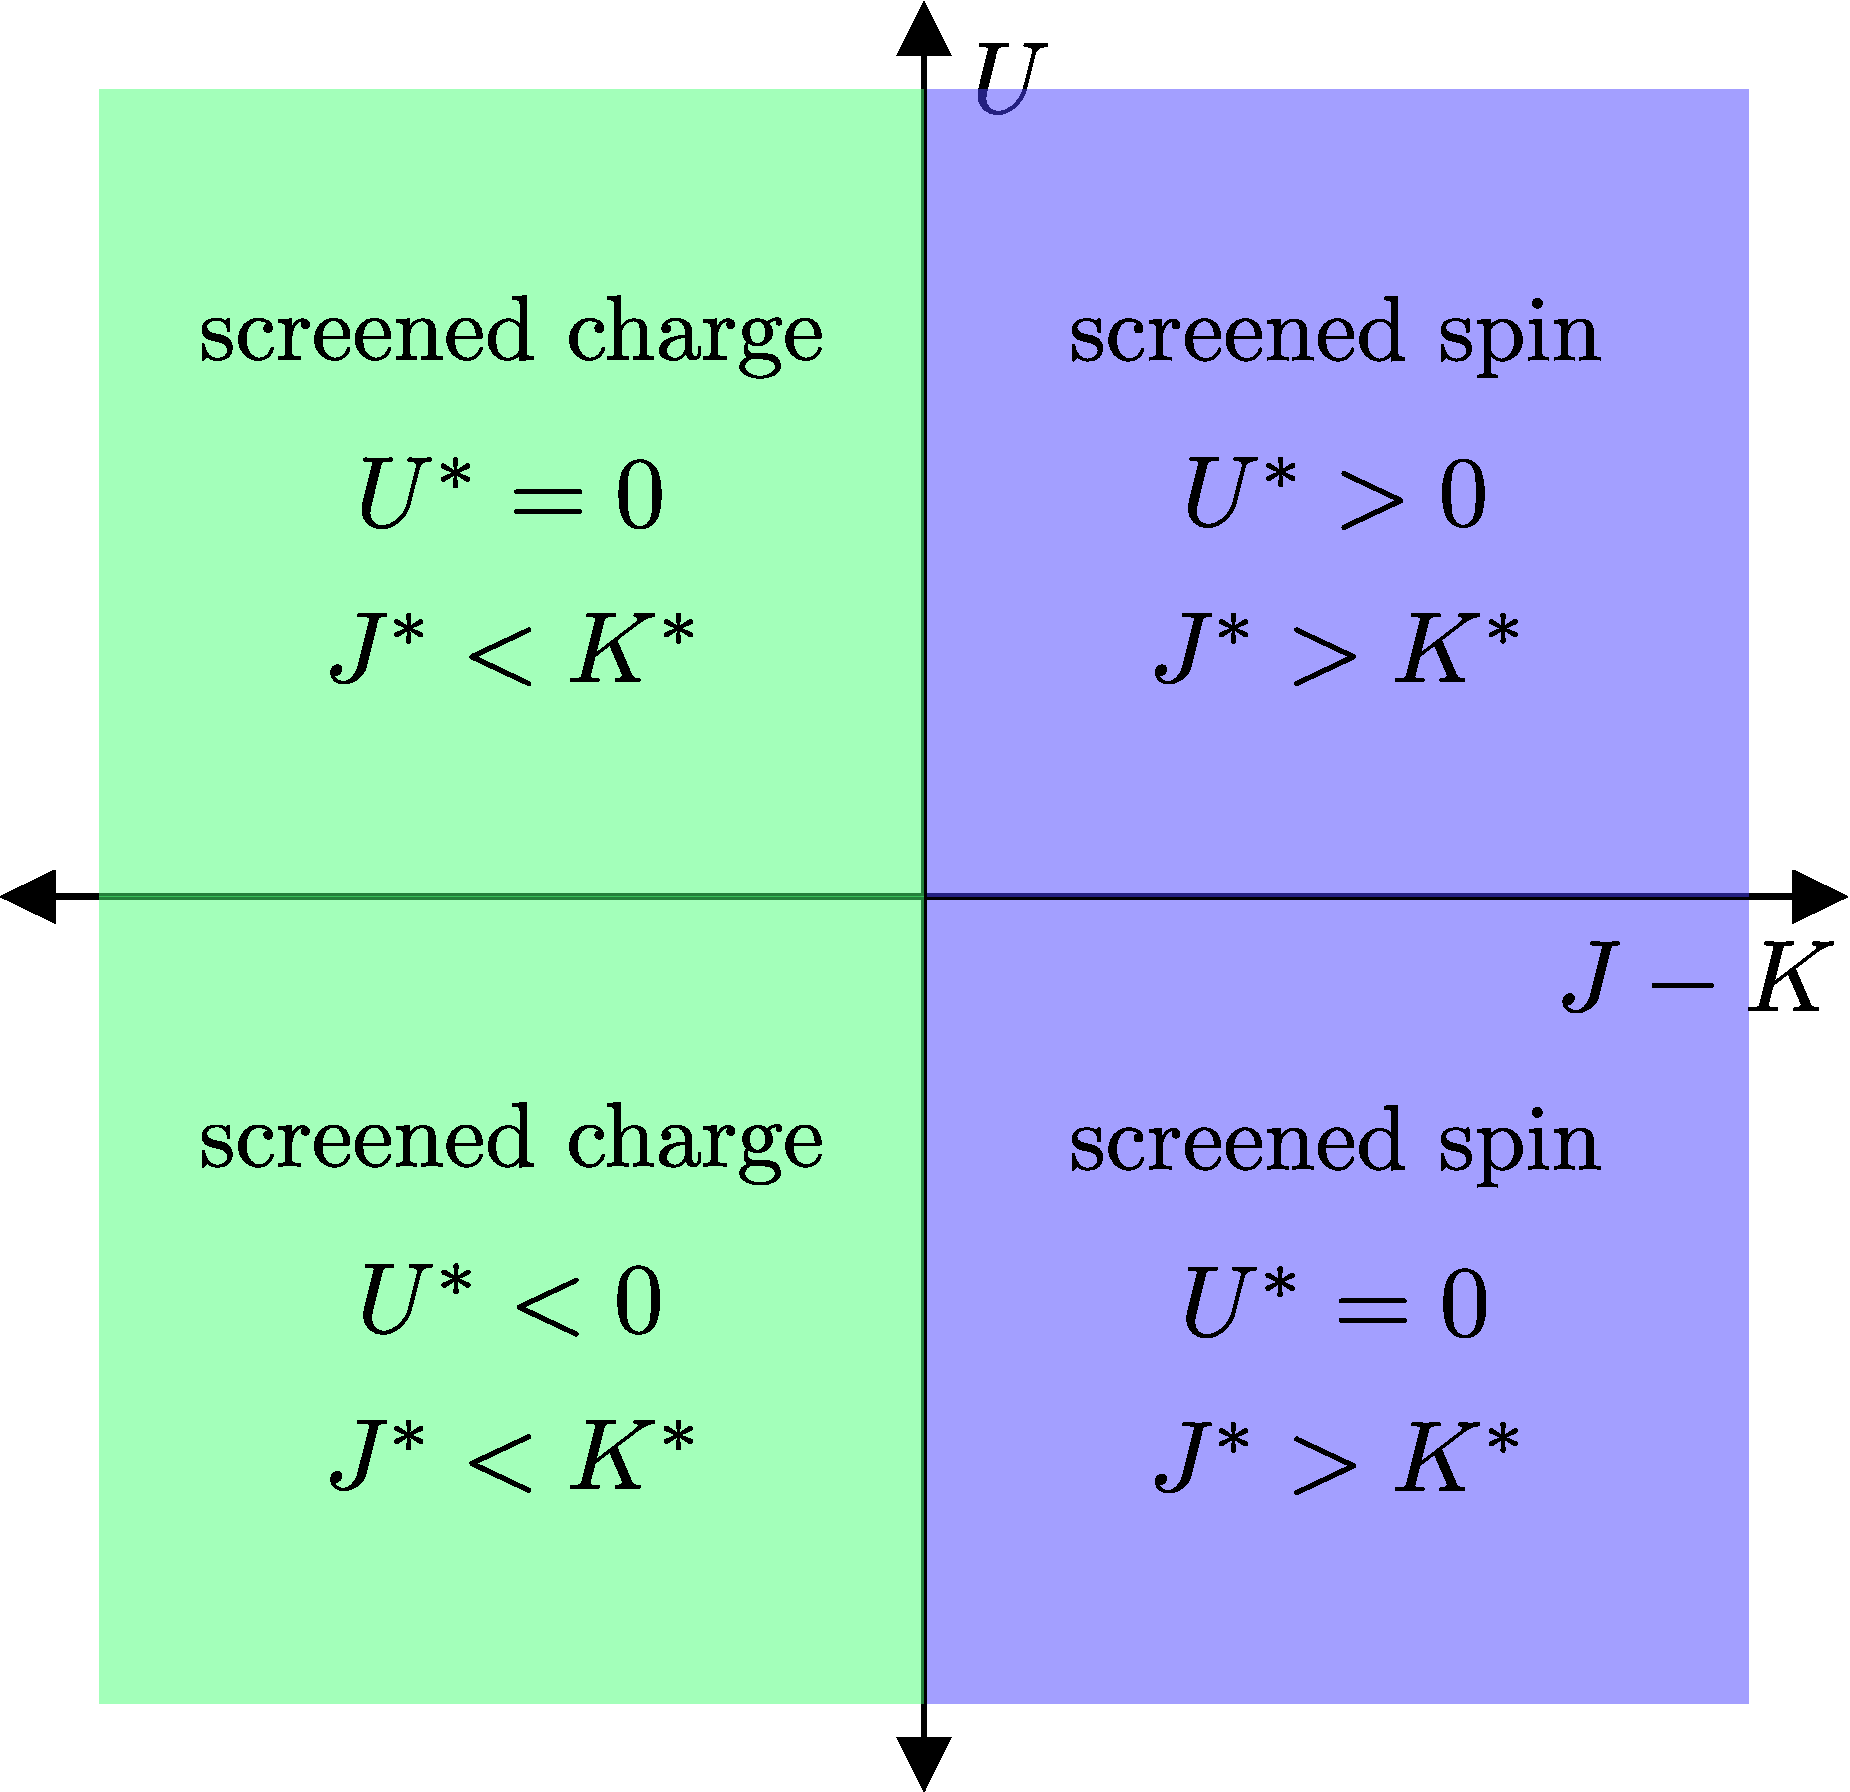
\includegraphics[scale=0.2]{../figures/phases.pdf}
	\caption{Fixed point phases in the plane of bare couplings, at \(V=0\).}
	\label{siamphases}
\end{figure}
\subsection{Effect of non-zero \(V\) on the RG flows}
The introduction of \(V\) into the RG equations make them analytically intractable, and we have to solve them numerically. The general observation is that we now get both zero and non-zero values of \(U^*\) in all the phases. The low quantum fluctuation scale behaviour in the first quadrant is shown in fig.~\ref{Veffect}. It is very similar to that obtained from NRG, as was shown in fig.~\ref{nrg_fp}.
\begin{figure}[!htb]
	\centering
	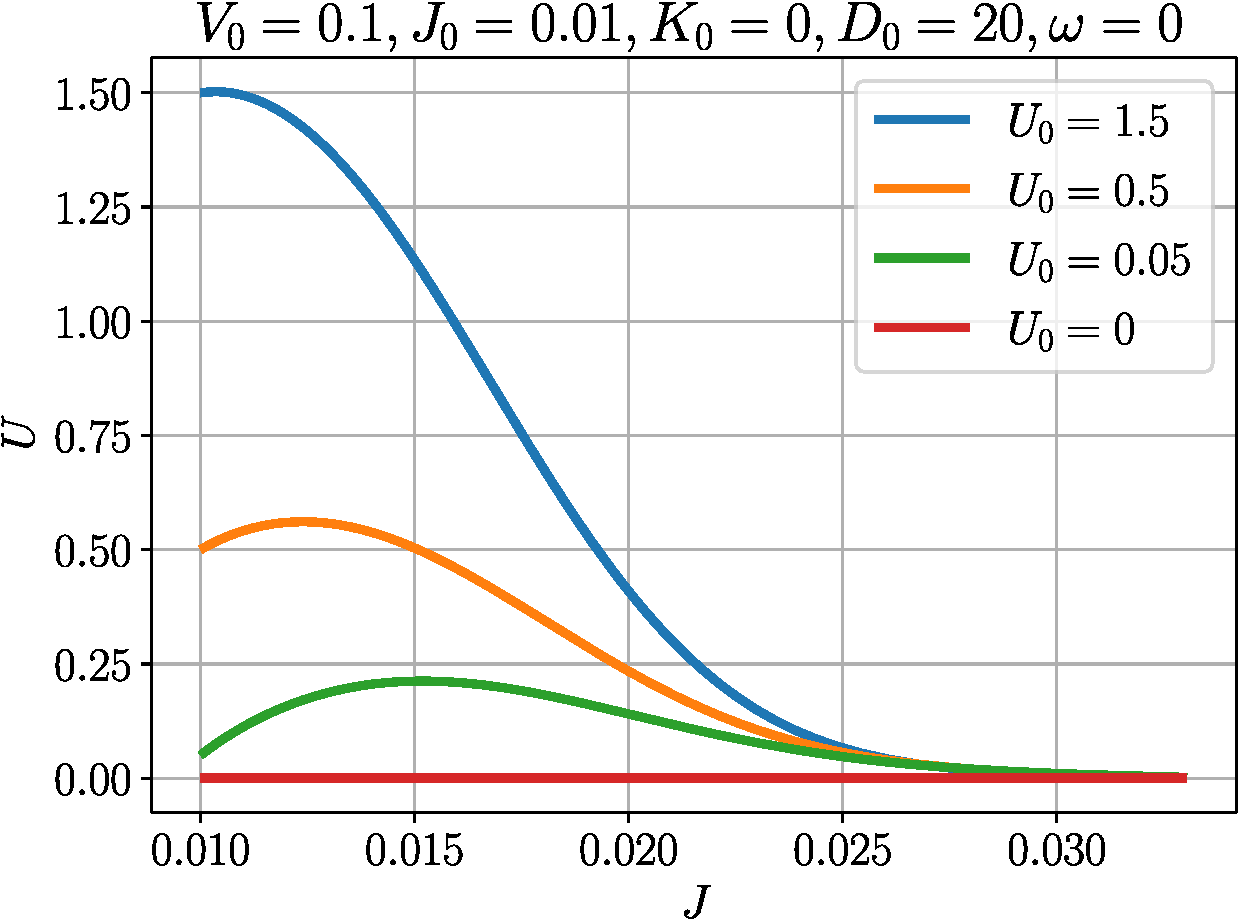
\includegraphics[width=0.6\textwidth]{../figures/UvsJ_new.pdf}
	\caption{\(U-J\) multiple RG flows in first quadrant.}
	\label{Veffect}
\end{figure}

\begin{figure}[!htb]
	\centering
	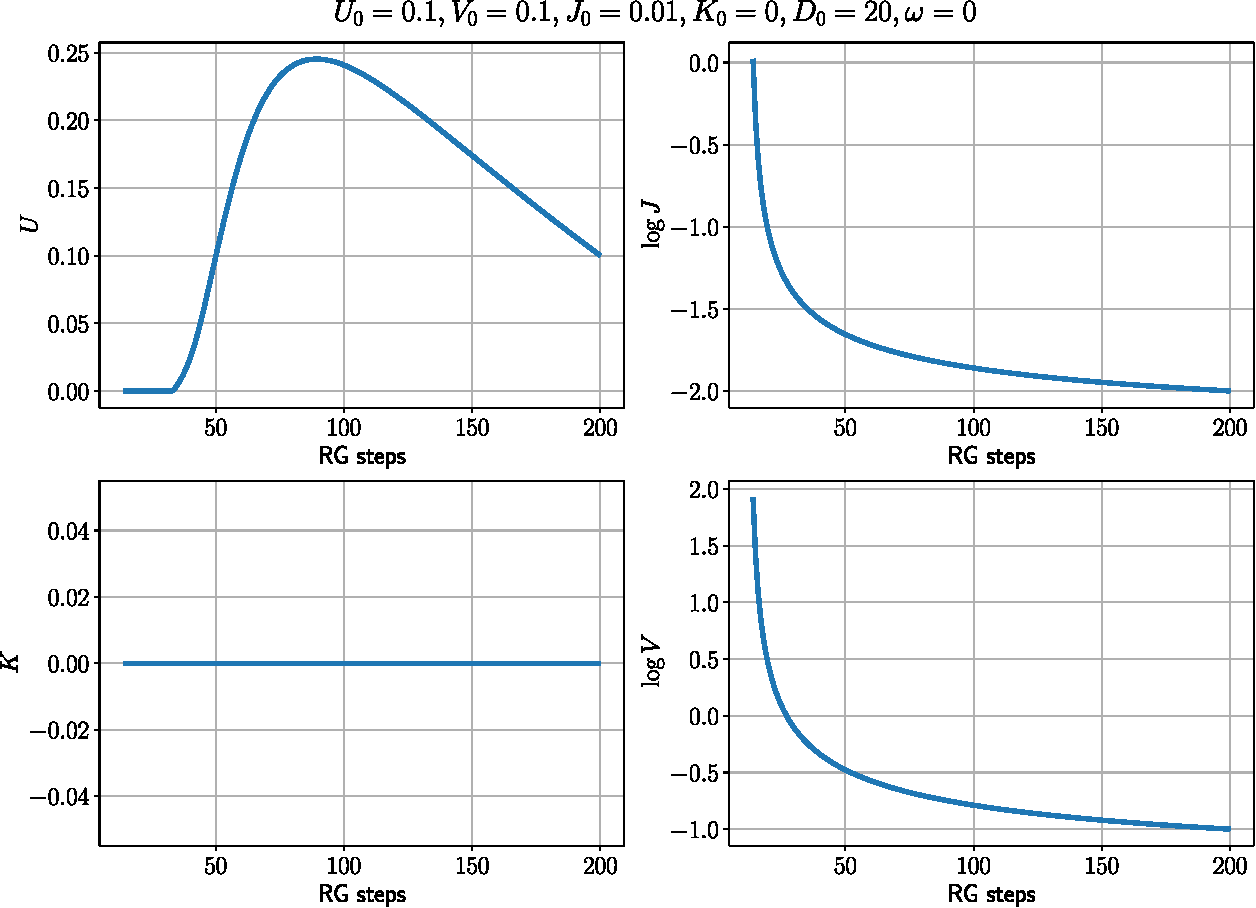
\includegraphics[width=0.8\textwidth]{../figures/with_V_new.pdf}
	\caption{Flows of the couplings for bare values in the first quadrant: \(J-K,U>0\).}
	% \label{Veffect}
\end{figure}
\paragraph*{First quadrant}
The first quadrant shows the flow from a free orbital fixed point near \(V=U=J=0\) to an intermediate local moment phase with large \(U\) with a final crossover to a stable fixed point at \(J^* \gg J_0, U^*=0\). The initial free orbital fixed point involves four degenerate impurity states at the impurity, and hence no local moment. The intermediate phase involves a local moment because of the large \(U\). The final stable phase involves an impurity which is strongly-coupled to the impurity because of the large \(V\) and \(J\). This crossover is depicted in fig.~\ref{crossover}.


\begin{figure}[!htb]
	\centering
	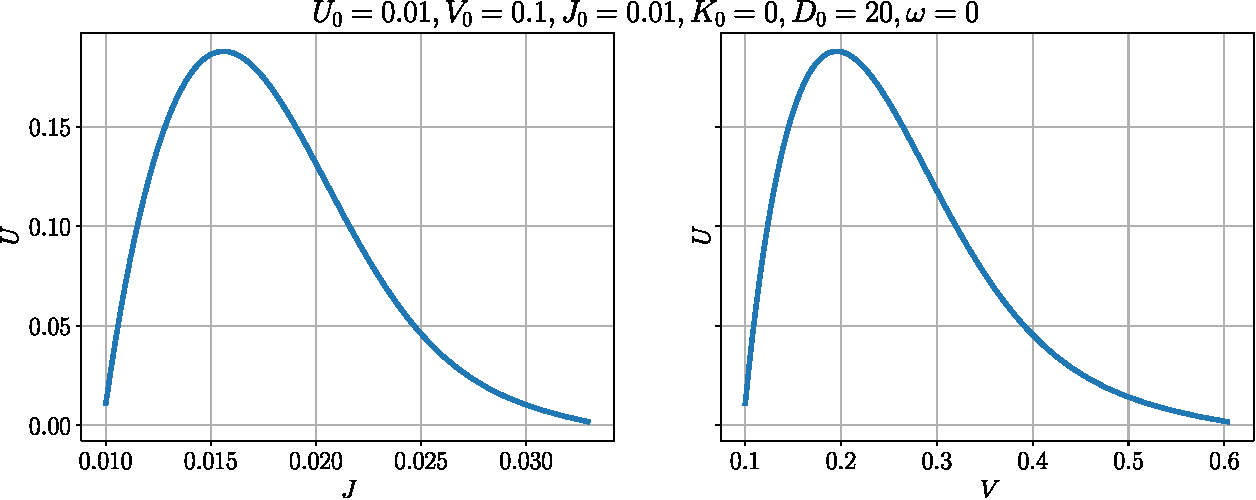
\includegraphics[width=0.8\textwidth]{../figures/crossovers_new.pdf}
	\caption{\(U-J\) and \(U-V\) RG flows.}
	\label{crossover}
\end{figure}

We have also checked that the fixed point values of \(J\) and \(V\) go on increasing as we increase the system size.

\begin{figure}[!htb]
	\centering
	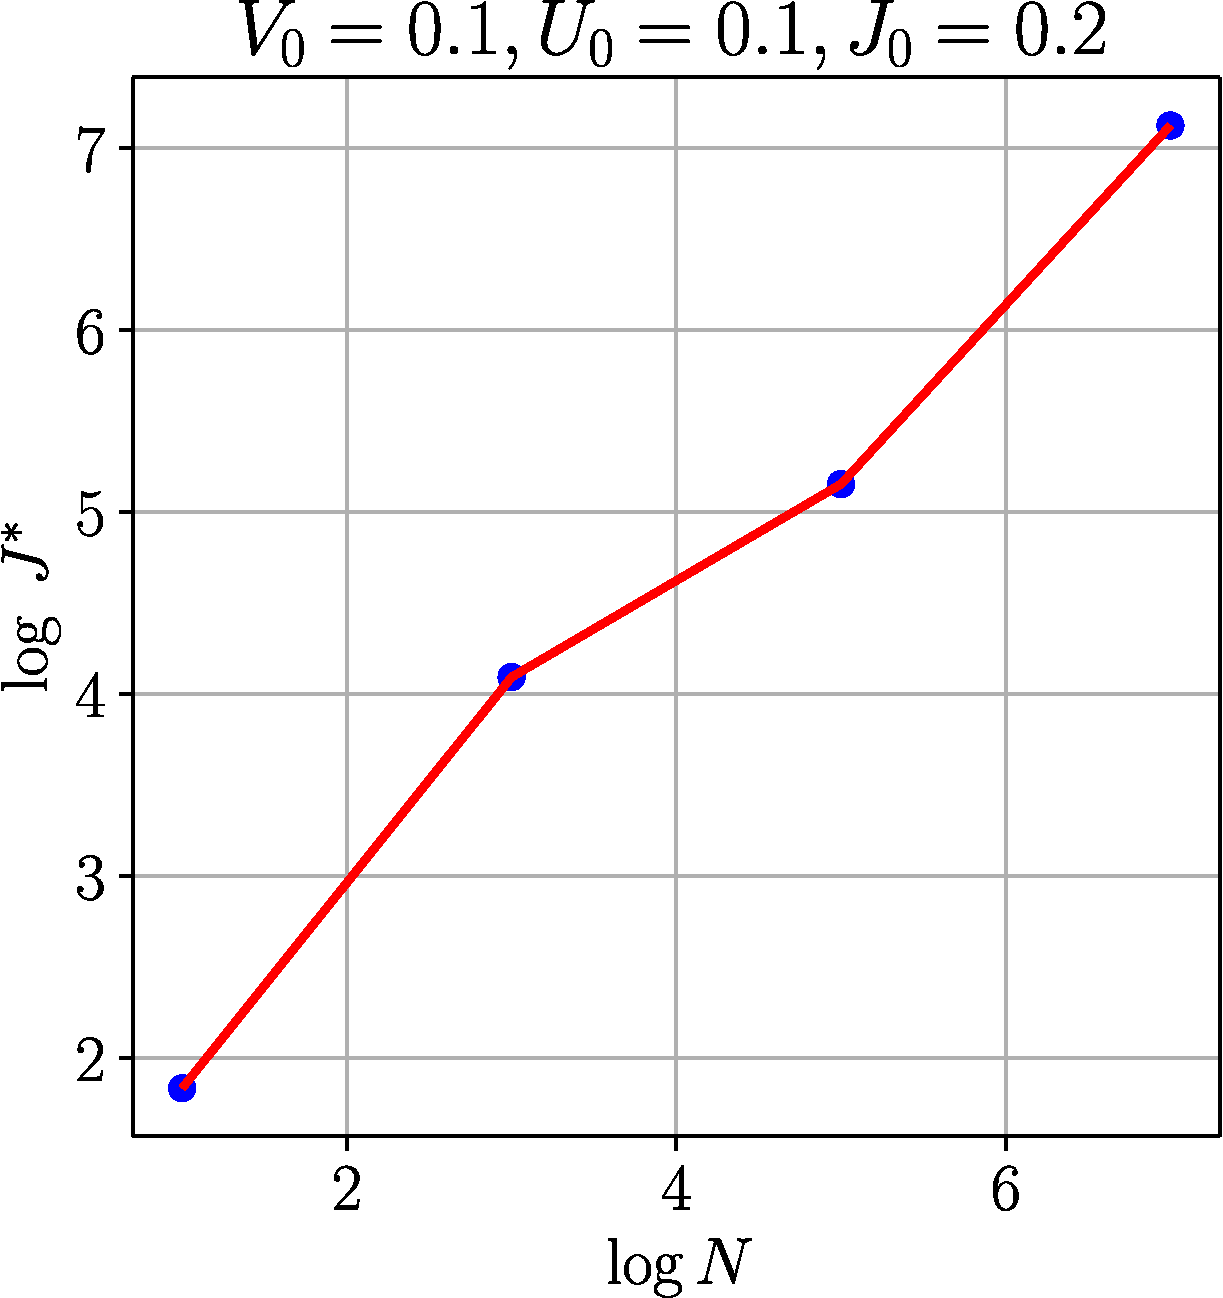
\includegraphics[width=0.4\textwidth]{../figures/J_vs_D_q1.pdf}
	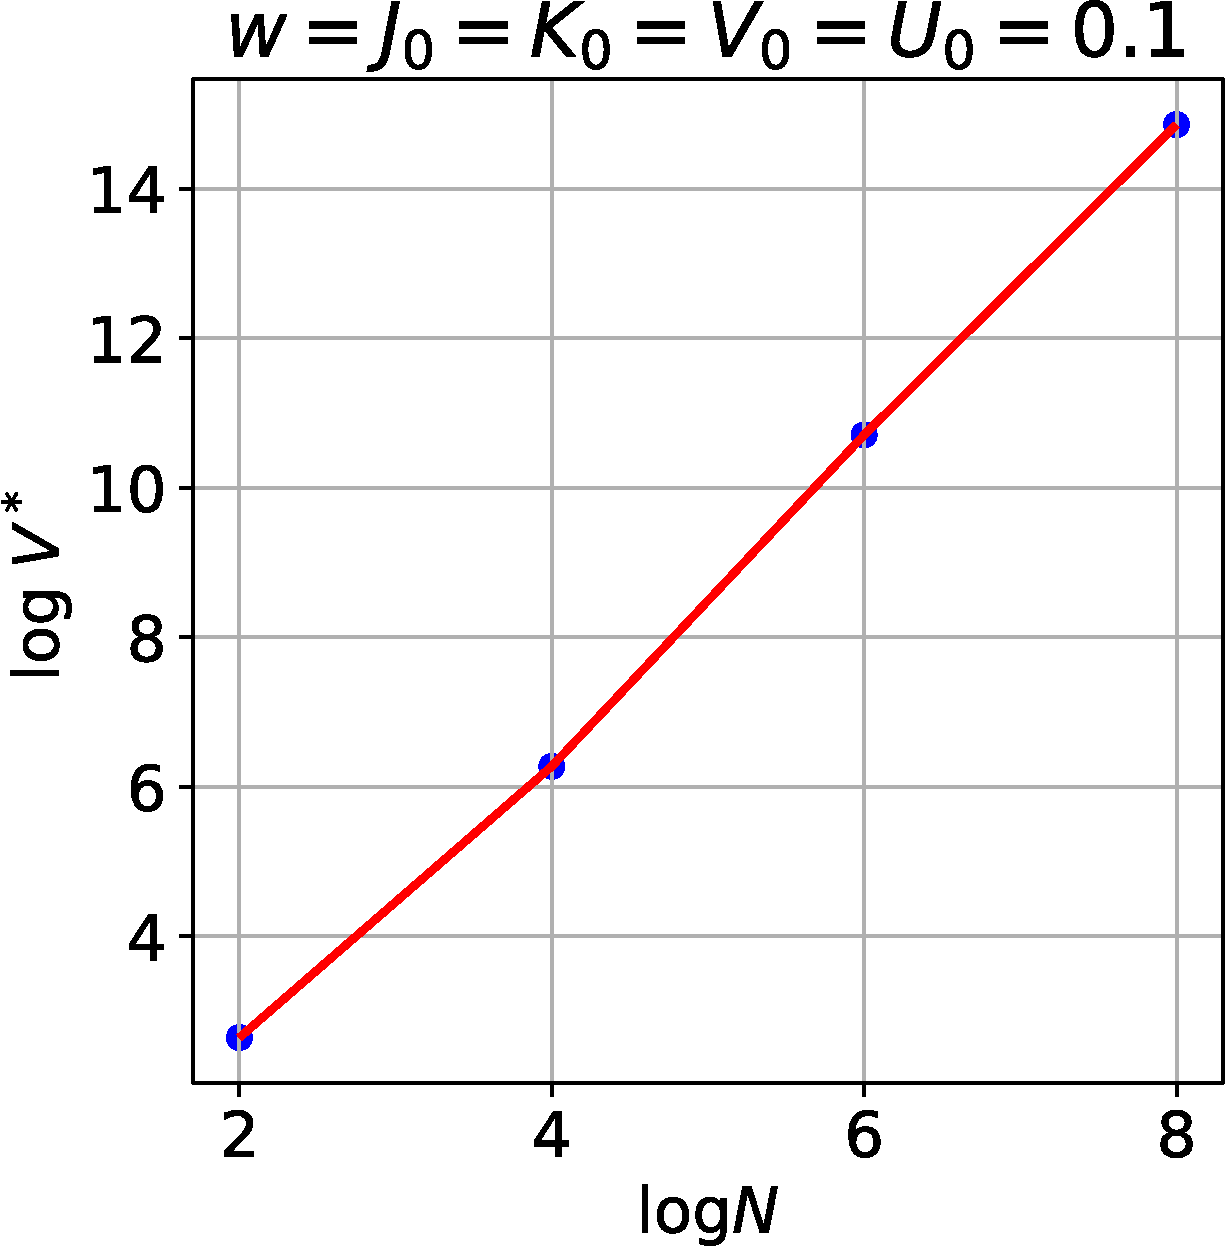
\includegraphics[width=0.4\textwidth]{../figures/V_vs_D_q1.pdf}
	\caption{Increase in the fixed point values of \(J\) and \(V\) with system size.}
	\label{JV-system-size}
\end{figure}
\paragraph*{Third quadrant}
In the third quadrant (\(U_0 < 0, K_0 > J_0\)), we see the flow to large negative value of \(U\), leading to a large contribution of the holon-doublon sectors of the impurity subspace, and a large value of \(K^*\) which means that the impurity charge sector couples very strongly with the bath charge sector.
\begin{figure}[htb!]
\centering
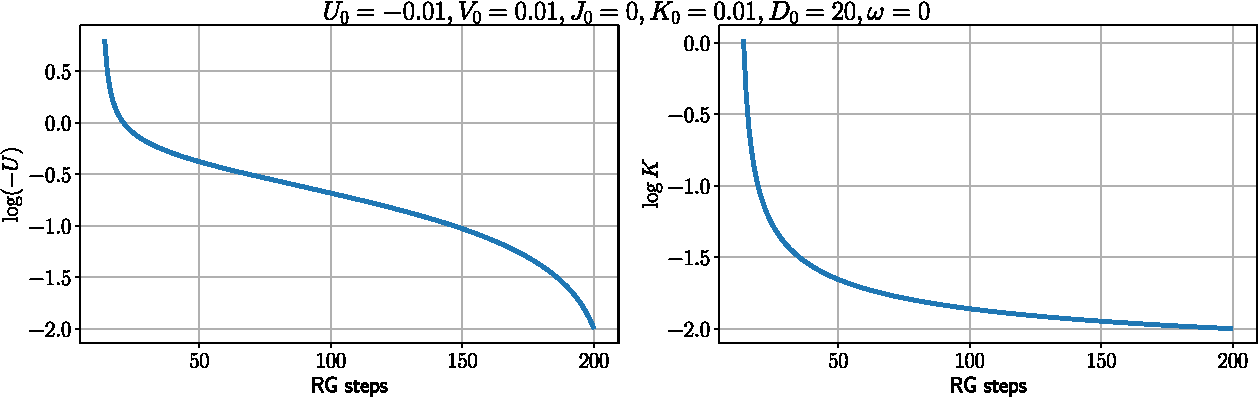
\includegraphics[width=0.8\textwidth]{../figures/with_V_q3_new.pdf}
\caption{Flow of \(U\) to large negative value and \(K\) to large positive value in the third quadrant.}
\label{frac_q3}
\end{figure}
This is essentially the charge analogue of the Kondo effect; the relevant transformation is
\begin{equation}\begin{aligned}
	\ket{\uparrow} \to \ket{2}, \ket{\downarrow} \to \ket{0}, J \to K, U \to -U
\end{aligned}\end{equation}
The ground state in this sector will be a charge singlet, as shown in the next section. This was also reported by Taraphder and Coleman in \cite{taraphder}.
\subsection{Phase diagram for \(V > 0\)}
We can now summarize the various fixed point phases. The physically relevant ones are the first and third quadrants. The first quadrant features a large spin-exchange coupling \(J\) and a positive \(U\) in the bare model, and the stable flows are towards a large \(J^*\) and a very small (\(\approx 0\)) \(U^*\). The fixed point state will be mostly a spin singlet, in which the impurity polarization gets quenched by the spin-flip scattering of the conduction electrons. The third quadrant is the regime of the charge-Kondo effect, and involves a negative \(U\) at the bare level which physically motivates a large charge-Kondo coupling \(K\). The fixed point again involves flow to a large \(K^*\), but the \(U\) flows to large negative here, implying a state where the charge sectors dominate heavily and the ground state is primarily a charge-singlet in which the destruction or annihilation of the Cooper-pair like states becomes prohibited.

These results are summarized in the table below.
\begin{table}[!htb]
\centering
\begin{tabular}{|c|c|c|c|c|c|c|}
\hline
\(U \) & \(J,K \) & \(U^*\) &\(J^*,K^*\) & class & ground state \\
\hline
\(>0\)& \(J > K\)& \(\gtrsim 0\)&\(J^*>K^*\) & screened spin & spin singlet + charge triplet\\
\(>0\)& \(J < K\)& \(\gtrsim 0\) &\(J^*<K^*\) & screened charge & charge singlet\\
\(<0\)& \(J > K\)& \(\gtrsim 0\) &\(J^*>K^*\) & screened spin & spin singlet + charge triplet\\
\(<0\)& \(J < K\)& \(\ll 0\)&\(J^*<K^*\) & screened charge & charge singlet\\
\hline
\end{tabular}
\caption{Classification of fixed points for various bare values, at \(V > 0\)}
\end{table}

\begin{figure}[!htb]
	\centering
	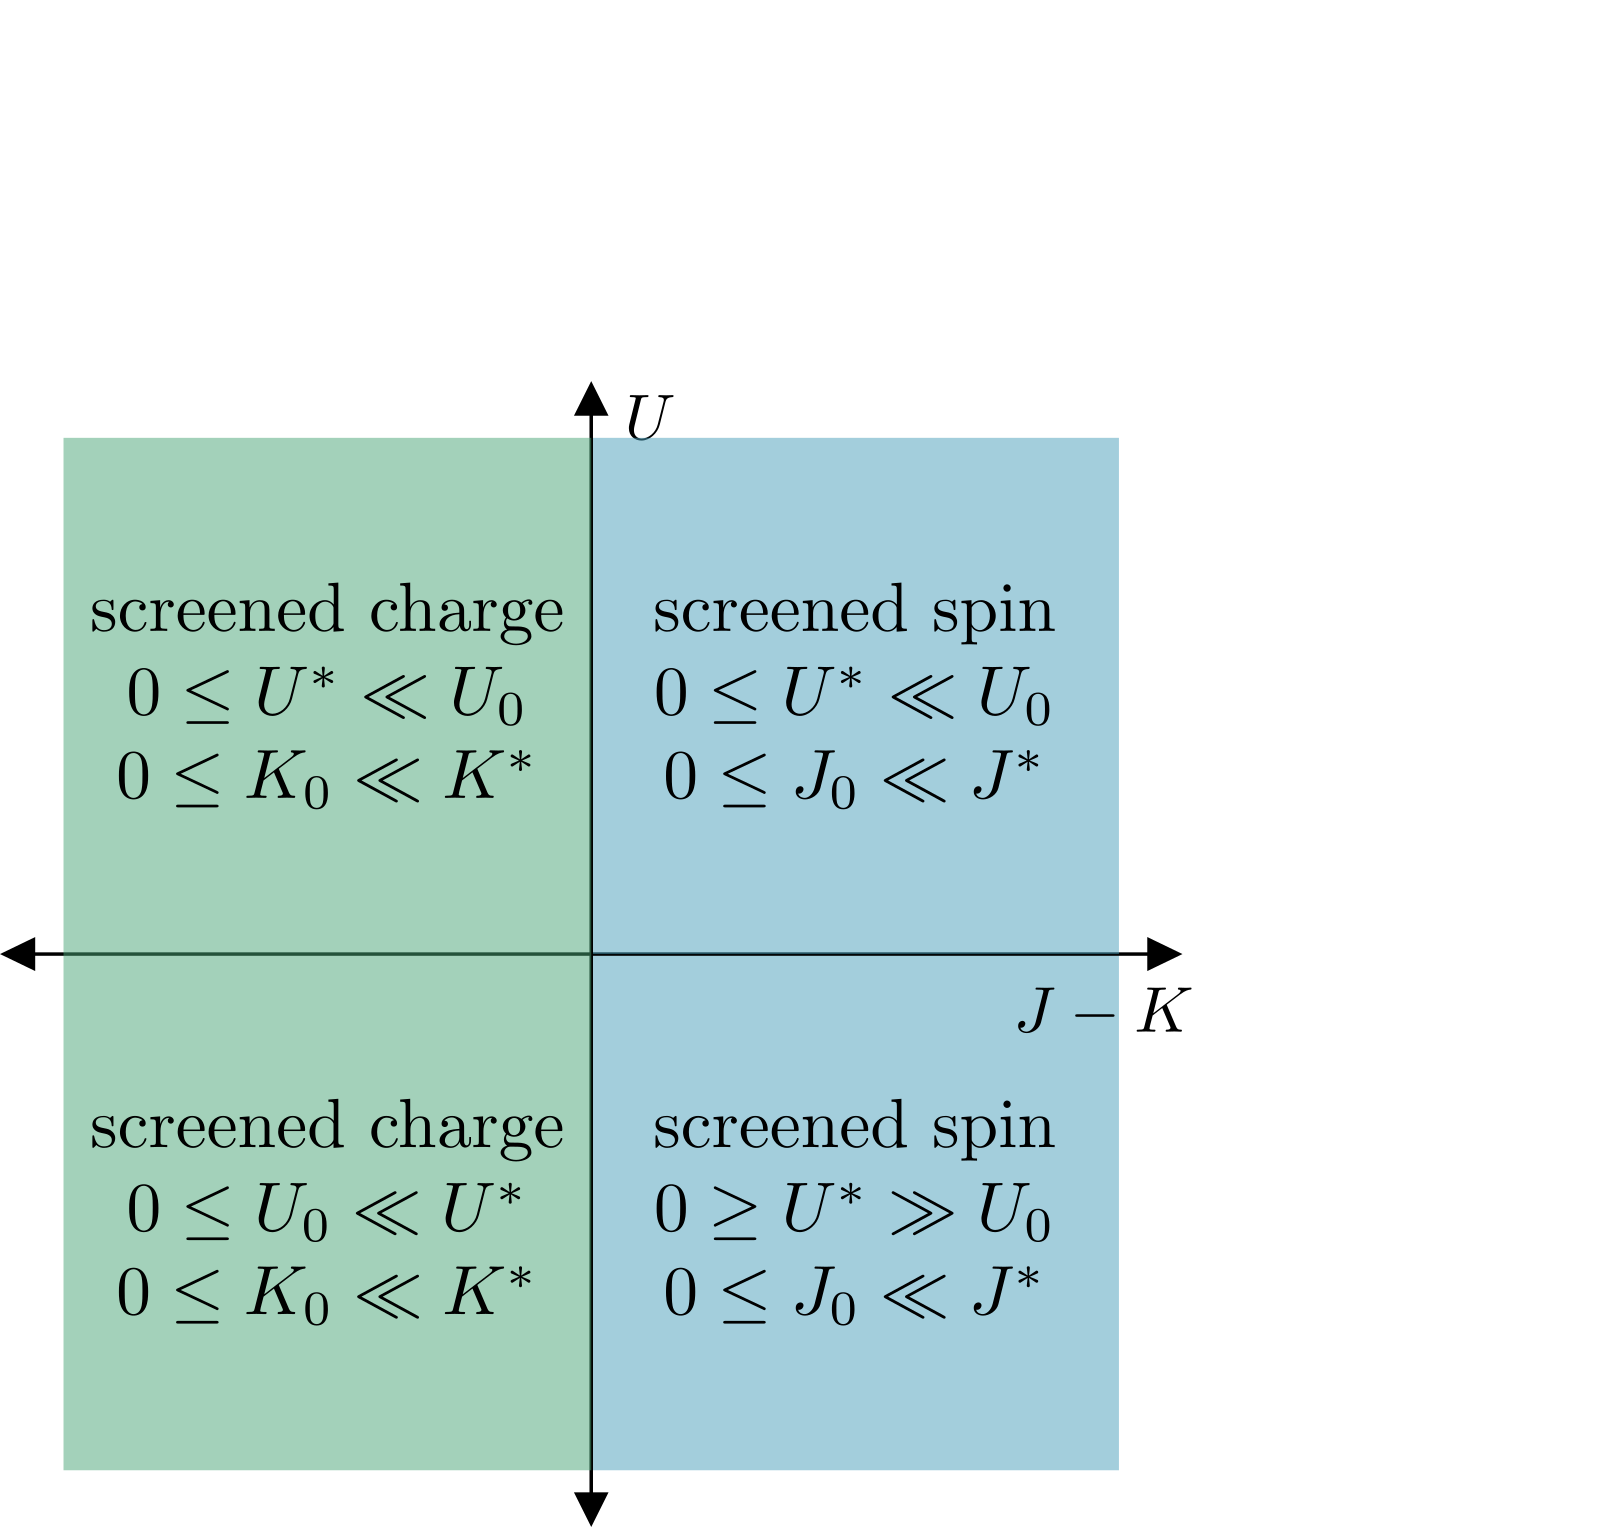
\includegraphics[width=0.4\textwidth]{../figures/phases_V.png}
	\caption{Low \(\omega\) fixed point phases for the SIAM with \(V>0\).}
\end{figure}

\section{Effective Hamiltonian and ground state for the \(V\neq 0\) symmetric problem}
The fixed point Hamiltonian can be written, in general, as
\begin{equation}\begin{aligned}
	\mathcal{H}^* = \sum_{\sigma, k}\epsilon_k \tau_{k\sigma} - \frac{U^*}{2}\hat n_d + U^* \hat n_{d\uparrow}\hat n_{d\downarrow} + \sum_{\sigma, k < \Lambda^*}\left( V^* c^\dagger_{k\sigma}c_{d\sigma} + \text{h.c.} \right) + J^* \vec{S_d}\cdot\vec{s} + K^* \vec{C_d}\cdot\vec{C} \\
	+ \sum_{q > \Lambda^*}\left(J^z_q S^z_ds^z_q + K^z_q C^z_dC^z_q\right) 
\end{aligned}\end{equation}
The first term is the kinetic energy of all the electrons. The next two terms are the impurity-diagonal pieces, featuring the renormalised interaction \(U^*\). The next three terms are the residual interactions between the impurity and the metal, with the renormalised couplings \(V^*, J^*\) and \(K^*\). The summations in these terms extend from the fixed point momentum cutoff \(\Lambda^*\) to 0. This is the region of momentum space  which the URG was unable to decouple. The operators \(\vec s\) and \(\vec C\) represent the macroscopic magnetic and charge spins formed by the remaining electrons that are lying inside the window \(\left[ 0, \Lambda^* \right] \):
\begin{equation}\begin{aligned}
	\vec s = \sum_{kk^\prime<\Lambda^*\atop{\alpha\beta}} c^\dagger_{k\alpha}\vec \sigma_{\alpha\beta}c_{k^\prime\beta}
\end{aligned}\end{equation}
The final two terms represent the diagonal pieces of the RG steps that have been completed. These survive because the URG removes only the number-off-diagonal terms; terms like \(S^d_z s_z\) and \(C^d_z C_z\) conserve the number of particles and hence survive. These will also be renormalised, and hence the subscript \(q\) on \(J^z_q\) signifies that it is has been renormalised up to a certain momentum.

Our goal here is to write down the ground state wavefunction for the low-energy Hamiltonian
\begin{equation}\begin{aligned}
	\label{fixed_point_ham}
	\mathcal{H}_{IR} = \sum_{\sigma, k<\Lambda^*}\epsilon_k \tau_{k\sigma} - \frac{U^*}{2}\hat n_d + U^* \hat n_{d\uparrow}\hat n_{d\downarrow} + \sum_{\sigma, k < \Lambda^*}\left( V^* c^\dagger_{k\sigma}c_{d\sigma} + \text{h.c.} \right) + J^* \vec{S_d}\cdot\vec{s} + K^* \vec{C_d}\cdot\vec{C}
\end{aligned}\end{equation}
To make progress with the ground state, we will simplify the effective Hamiltonian by mapping it onto a two-site problem. One site is of course the impurity site. The other site will be formed by the centre of mass degree of freedom of the conduction electrons, which we define as
\begin{equation}\begin{aligned}
	c_{2\sigma} \equiv \frac{1}{\sqrt{N^*}}\sum_{k} c_{k\sigma} = c_\sigma\left( \vec r = 0 \right) 
\end{aligned}\end{equation}
where \(N^*\) is the number of electrons inside the window \(\left[-\Lambda^*, \Lambda^*\right]\). This operator essentially creates a conduction electron at the origin. It is easy to prove that this operator is Fermionic:
\begin{equation}\begin{aligned}
	\label{site2antic}
	\left\{c_{2\sigma}, c^\dagger_{2\sigma} \right\}  &= \frac{1}{N^*}\sum_{kk^\prime} \left\{ c_{k\sigma}, c^\dagger_{k^\prime\sigma} \right\} = \frac{1}{N^*}\sum_{kk^\prime} \delta_{kk^\prime} = 1\\
	\left\{c_{2\sigma}, c_{2\sigma} \right\}  &= \frac{1}{N^*}\sum_{kk^\prime} \left\{ c_{k\sigma}, c_{k^\prime\sigma} \right\} = 0
\end{aligned}\end{equation}
The number operator corresponding to this degree of freedom is
\begin{equation}\begin{aligned}
	\hat n_{2\sigma} = c^\dagger_{2\sigma}c_{2\sigma} = \frac{1}{N^*}\sum_{kk^\prime}c^\dagger_{k\sigma}c_{k^\prime\sigma}
\end{aligned}\end{equation}
Because of the anticommutation algebra in eq.~\ref{site2antic}, this operator behaves essentially like a Fermion: \(\hat n_{2\sigma}^2 = \hat n_{2\sigma}\). For our two-site problem, we will imagine this to be the annihilation operator for the site 2, for the spin sigma. The corresponding operator for the first site is of course just the impurity electron annihilation operator:
\begin{equation}\begin{aligned}
	c_{1\sigma} \equiv c_{d\sigma}
\end{aligned}\end{equation}
The various terms of the Hamiltonian can now be written in terms of these operators. We write the Fourier decomposition of the dispersion of the conduction bath.
\begin{equation}\begin{aligned}
	\epsilon_{\vec{k}} = \frac{1}{N^*}\sum_{\vec r}e^{i \vec{k}\cdot\vec{r}}\epsilon(\vec r)
\end{aligned}\end{equation}
The inverse transformation is
\begin{equation}\begin{aligned}
	\epsilon(\vec r) = \sum_{|\vec k| < \Lambda^*}e^{-i \vec{k}\cdot\vec{r}}\epsilon_{\vec{k}}
\end{aligned}\end{equation}
We now make a simplifying assumption: Guided by the observation that the important degree of freedom at the fixed point is the COM operator \(c_{2\sigma}\), we keep only the \(\vec r=0\) mode of the decomposition:
\begin{equation}\begin{aligned}
	\epsilon_{\vec k} \approx \frac{1}{N^*}\epsilon(\vec r=0) = \frac{1}{N^*}\sum_{k<\Lambda^*}\epsilon_k = \frac{1}{N^*}\sum_{\epsilon_k \in [\epsilon_F - D^*, \epsilon_F + D^*]}\epsilon_k = \epsilon_F
\end{aligned}\end{equation}
\(\epsilon_F\) is the Fermi energy, which we henceforth set to 0. The energy term for the second site is thus simply zero. The impurity diagonal part of \(\mathcal{H}_{IR}\) will survive only when \(\hat n_d = \hat n_1 = 1\). So we write it as
\begin{equation}\begin{aligned}
	- \frac{U^*}{2}\hat n_d + U^* \hat n_{d\uparrow}\hat n_{d\downarrow} = - \frac{U^*}{2}\left(\hat n_{d\uparrow} + \hat n_{d \downarrow} - 2\hat n_{d\uparrow}\hat n_{d\downarrow}\right) = - \frac{U^*}{2} \left(\hat n_{1 \uparrow} - \hat n_{1 \downarrow}\right)^2 \equiv \epsilon_d \left(\hat n_{1 \uparrow} - \hat n_{1 \downarrow}\right)^2
\end{aligned}\end{equation}
where \(\epsilon_d = - \frac{U^*}{2}\). The off-diagonal terms can also be similarly transformed into a two-site problem. The bath spin can be written as
\begin{equation}\begin{aligned}
	\vec S_d &\equiv \vec S_1\\
	J^*\vec s &= J^* \frac{1}{2}\sum_{kk^\prime\atop{\alpha\beta}}c^\dagger_{k\alpha}\vec \sigma_{\alpha\beta}c_{k^\prime\beta} \\
	       &= J^*\frac{1}{2}\sum_{\alpha\beta}c^\dagger_{2\alpha}\vec \sigma_{\alpha\beta}c_{2\beta} \\
	       &= J^* N^* \frac{1}{2}\left[\hat z\left(c^\dagger_{2 \uparrow}c_{2 \uparrow} - c^\dagger_{2 \downarrow} c_{2 \downarrow} \right) + \hat x \left(c^\dagger_{2 \uparrow}c_{2 \downarrow} + c^\dagger_{2 \downarrow} c_{2 \uparrow} \right) -i \hat y \left( c^\dagger_{2 \uparrow}c_{2 \downarrow} - c^\dagger_{2 \downarrow} c_{2 \uparrow} \right)\right]\\
	       &\equiv J^*N^* \vec S_2\\
	       &\equiv j \vec S_2\\
\end{aligned}\end{equation}
where \(j \equiv J^* N^*\) and
\begin{equation}\begin{aligned}
	\vec S_2 = \frac{1}{2N^*}\sum_{kk^\prime\atop{\alpha\beta}}c^\dagger_{k\alpha}\vec \sigma_{\alpha\beta}c_{k^\prime\beta}
\end{aligned}\end{equation}
. The charge isospins can also be rewritten similarly. From eq.~\ref{diagonalCz},
\begin{equation}\begin{aligned}
	K^* C^z &=K^* \frac{1}{2}\sum_{kk^\prime}\left( c^\dagger_{k \uparrow}c_{k^\prime \uparrow} - c_{k^\prime \downarrow}c^\dagger_{k \downarrow} \right) = \frac{1}{2}N^* K^*\left( c^\dagger_{2 \uparrow}c_{2 \uparrow} - c_{2 \downarrow}c^\dagger_{2\downarrow} \right) = kC_2^z\\
	K^* C^x &=K^* \frac{1}{2}\sum_{kk^\prime}\left( c^\dagger_{k \uparrow}c^\dagger_{k^\prime \downarrow} + c_{k \downarrow}c^\dagger_{k^\prime \uparrow} \right) = \frac{1}{2}N^* K^*\left( c^\dagger_{2 \uparrow}c_{2 \downarrow} - c_{2 \downarrow}c^\dagger_{2\uparrow} \right) = kC_2^x\\
\end{aligned}\end{equation}
and similarly for \(C^y\). We defined \(k \equiv K^* N^*\). The diagonal component \(C^z\) can also be written as
\begin{equation}\begin{aligned}
	 C^z = \frac{1}{2}N^* \sum_\sigma\left(c^\dagger_{2\sigma}c_{2\sigma} - \frac{1}{2}\right) = \frac{1}{2}N^*\tau_2
\end{aligned}\end{equation}
where \(\tau_2 = \sum_\sigma \tau_{2\sigma} = \sum_\sigma \left( \hat n_{2\sigma} - \frac{1}{2} \right) \). The hybridisation term can be written as
\begin{equation}\begin{aligned}
	V\sum_k c^\dagger_{k\sigma} = V\sqrt{N^*} c^\dagger_{2\sigma} = vc^\dagger_{2\sigma}
\end{aligned}\end{equation}
where \(v \equiv V\sqrt{N^*}\). The charge isospins can be written down similarly. Combining these, the interaction part can be written as
\begin{equation}\begin{aligned}
v\sum_{\sigma}\left( c^\dagger_{1\sigma}c_{2\sigma} + \text{h.c.} \right) + j\vec{S_1}\cdot\vec{S_2} + k\vec{C_1}\cdot\vec{C_2}
\end{aligned}\end{equation}
with \(k = K^* N^*\). The total Hamiltonian for the two-site problem is
\begin{equation}\begin{aligned}
	\mathcal{H}_{IR} = \epsilon_d m_1^2 + v\sum_{\sigma}\left(c^\dagger_{1\sigma}c_{2\sigma} + \text{h.c.} \right) + j\vec{S_1}\cdot\vec{S_2} + k \vec{C_1}\cdot\vec{C_2}
\end{aligned}\end{equation}
where we have dropped the \(*\) on the couplings for brevity and \(\hat n_{1 \uparrow} - \hat n_{1 \downarrow}=m_1\) is the magnetization on the first site. We will use the following notation to represent kets of this two-site system: \(\ket{n_{1 \uparrow}n_{1 \downarrow}n_{2 \uparrow}n_{2 \downarrow}}\). For example, a state \(\ket{1001}\) represents a ket with an up electron on site 1 and a down electron on site 2. This Hamiltonian conserves the total number operator \(\hat n \equiv \hat n_1 + \hat n_2\), so we can analyse the various subspaces corresponding to particular values of \(\hat n\) separately.
\begin{figure}[!htb]
	\centering
	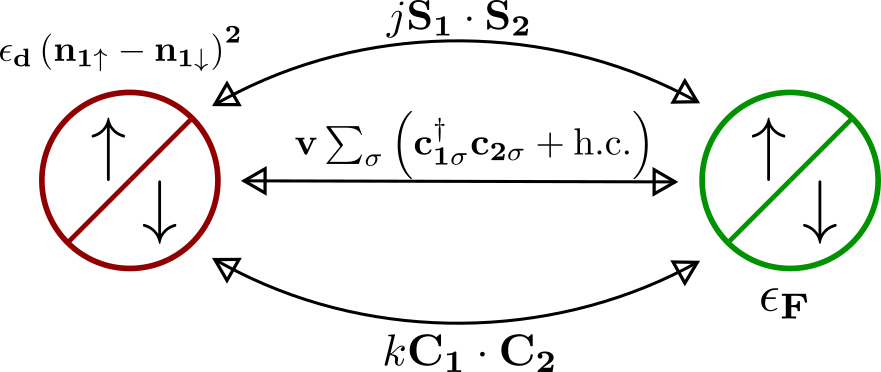
\includegraphics[width=0.4\textwidth]{../figures/two_site_problem.png}
	\caption{Two-site effective problem of fixed point Hamiltonian}
	\label{twosite}

\end{figure}

We will adopt the following notation to represent the states in this Hilbert space. A general state will be represented in the Fock space basis as \(\ket{n_{1 \uparrow}n_{1 \downarrow}n_{2 \uparrow}n_{2 \downarrow}}\). For example,
\begin{equation}\begin{aligned}
	\ket{1101} = c^\dagger_{1 \uparrow}c^\dagger_{1 \downarrow}c^\dagger_{2 \downarrow}\ket{-}
\end{aligned}\end{equation}
\(\ket{-}\) is the vacuum state.

First lets get the trivial cases of \(\hat n = 0, 4\) out of the way. The only possible states are \(\ket{0000}\) and \(\ket{1111}\) respectively. Both these states are eigenstates because the first one has no electron to scatter, and the second one has no vacant state to scatter into. These states have energy eigenvalues \( \frac{1}{4}k\)

The subspaces \(\hat n = 1,3\) are each four-dimensional. More precisely speaking, the \(\hat n=1\) subspace can have the following basis
\begin{equation}\begin{aligned}
	\ket{\uparrow,0}, \ket{0,\uparrow}, \ket{\downarrow,0}, \ket{0,\downarrow}
\end{aligned}\end{equation}
However, since the Hamiltonian conserves the total spin (both magnetic and charge), we can divide this Hilbert subspace into two smaller subspaces which do not talk to each other - one having the states \(\ket{\uparrow,0}, \ket{0,\uparrow}\) and hence a total spin magnetization of \(+\frac{1}{2}\), and the other having the remaining states and a total spin magnetization of \(-\frac{1}{2}\). The action of the Hamiltonian on this subspace is
\begin{equation}\begin{aligned}
	\mathcal{H}_{IR} \ket{1000} &= \left[\epsilon_d m_1^2 + vc^\dagger_{2 \uparrow}c_{1 \uparrow}\right] c^\dagger_{1 \uparrow}\ket{-} = \epsilon_d\ket{1000} + v\ket{0010}\\
	\mathcal{H}_{IR} \ket{0010} &= \left[\epsilon_d m_1^2 + vc^\dagger_{1 \uparrow}c_{2 \uparrow}\right] c^\dagger_{2 \uparrow}\ket{-} = v\ket{1000}\\
\end{aligned}\end{equation}
The Hamiltonian in first subspace can be represented by the matrix
\begin{equation}\begin{aligned}
	\label{n1mat}
	\bordermatrix{~&\ket{\uparrow,0} & \ket{0,\uparrow} \\
		~&\epsilon_d & v \\
		~& v & 0 \\
	}
\end{aligned}\end{equation}
The eigenstates (un-normalised) are
\begin{equation}\begin{aligned}
\label{low}
	-4v\ket{\uparrow,0} +2 \left[ \epsilon_d \mp \Delta\left(\epsilon_d , v\right)\right] \ket{0, \uparrow}, && E^1_\pm = \frac{1}{2} \epsilon_d \pm \frac{1}{2}\Delta\left(\epsilon_d , v\right)
\end{aligned}\end{equation}
where \(\Delta\left(\epsilon_d , v\right)  = \sqrt{\epsilon_d^2 + 4 v^2}\). The other two eigenstates (corresponding to magnetization \(- \frac{1}{2}\) need not be calculated separately; since the Hamiltonian is invariant under the transformation \( \uparrow \leftrightarrow \downarrow\), we can do a similar transformation on the eigenkets to get the eigenkets for the other subspace.
\begin{equation}\begin{aligned}
	-4v\ket{\downarrow,0} + 2 \left[ \epsilon_d \mp \Delta\left(\epsilon_d , v \right)\right] \ket{0, \downarrow}
\end{aligned}\end{equation}
with exactly the same eigenvalue.

The \(\hat n = 3\) subspace is very similar. We can obtain the basis directly from the \(\hat n = 1\) case by substituting the holes with doubles:
\begin{equation}\begin{aligned}
	\ket{\uparrow,\uparrow \downarrow}, \ket{\uparrow \downarrow,\uparrow}, \ket{\downarrow,\uparrow \downarrow}, \ket{\uparrow \downarrow,\downarrow}
\end{aligned}\end{equation}
Since a double impurity has the same energy as a vacant impurity (because of p-h symmetry, both are zero), the diagonal part corresponding to the first site will not change. We can then write down the eigenstates and eigenvalues directly from those of \(\hat n=1\), simply by making the transformation \(\ket{0} \to \ket{ \uparrow \downarrow}\).
\begin{align}
	\left.
	\begin{array}{l}
	-4v \ket{\uparrow,\uparrow \downarrow} +  2\left[ \epsilon_d \mp \Delta\left(\epsilon_d , v\right)  \right] \ket{\uparrow \downarrow, \uparrow}\\
	-4v \ket{\downarrow,\uparrow \downarrow} + 2 \left[ \epsilon_d \mp \Delta\left(\epsilon_d, v\right)  \right] \ket{\uparrow \downarrow, \downarrow}\end{array}
	\right\}
	E = \frac{1}{2} \epsilon_d \pm \frac{1}{2}\Delta\left(\epsilon_d , v \right)
\end{align}
The most interesting subspace is \(\hat n=2\). This is six dimensional. Since the Hamiltonian conserves both the total spins \(S^2\) and \(C^2\) as well the z-components \(S^z = S_1^z + S^z_2\) and \(C^z = C_1^z + C^z_2\), it would be prudent to choose our basis with this in mind. The action of the hybridisation term on the various states are
\begin{equation}\begin{aligned}
	&v\left( c^\dagger_{1 \downarrow} c_{2 \downarrow} +  c^\dagger_{2 \uparrow} c_{1 \uparrow}\right) c^\dagger_{1 \uparrow}c^\dagger_{2 \downarrow}\ket{-} = v\left(c^\dagger_{1 \uparrow}c^\dagger_{1 \downarrow} c_{2 \downarrow}  c^\dagger_{2 \downarrow}+  c^\dagger_{2 \uparrow} c^\dagger_{2 \downarrow}c_{1 \uparrow} c^\dagger_{1 \uparrow}\right)\ket{-} = v \ket{\uparrow \downarrow,0}  + v \ket{0, \uparrow \downarrow}\\
	&v\left( c^\dagger_{1 \uparrow} c_{2 \uparrow} +  c^\dagger_{2 \downarrow} c_{1 \downarrow}\right) c^\dagger_{1 \downarrow}c^\dagger_{2 \uparrow}\ket{-} = v\left(-c^\dagger_{1 \uparrow}c^\dagger_{1 \downarrow} c_{2 \uparrow}  c^\dagger_{2 \uparrow} - c^\dagger_{2 \uparrow} c^\dagger_{2 \downarrow}c_{1 \downarrow} c^\dagger_{1 \downarrow}\right)\ket{-} = -v \ket{\uparrow \downarrow,0} -v \ket{0, \uparrow \downarrow}\\
	&v\left( c^\dagger_{2 \uparrow} c_{1 \uparrow} +  c^\dagger_{2 \downarrow} c_{1 \downarrow}\right) c^\dagger_{1 \uparrow}c^\dagger_{1 \downarrow}\ket{-} = v\left(-c^\dagger_{1 \downarrow}c^\dagger_{2 \uparrow} c_{1 \uparrow}  c^\dagger_{1 \uparrow} + c^\dagger_{1 \uparrow} c^\dagger_{2 \downarrow}c_{1 \downarrow} c^\dagger_{1 \downarrow}\right)\ket{-} = -v \ket{\downarrow, \uparrow} + v \ket{\uparrow, \downarrow} \\
	&v\left( c^\dagger_{1 \uparrow} c_{2 \uparrow} +  c^\dagger_{1 \downarrow} c_{2 \downarrow}\right) c^\dagger_{2 \uparrow}c^\dagger_{2 \downarrow}\ket{-} = v\left(c^\dagger_{1 \uparrow} c^\dagger_{2 \downarrow}c_{2 \uparrow} c^\dagger_{2 \uparrow}-c^\dagger_{1 \downarrow}c^\dagger_{2 \uparrow} c_{2 \downarrow}  c^\dagger_{2 \downarrow}\right)\ket{-} = v \ket{\uparrow, \downarrow} -v \ket{\downarrow, \uparrow}\\
\end{aligned}\end{equation}
\begin{flalign}
	\mathcal{H}_{IR}\ket{\uparrow, \uparrow} &= \left(\epsilon_d + \frac{1}{4}j\right)\ket{\uparrow, \uparrow} \label{1}\\
	\mathcal{H}_{IR}\ket{\downarrow, \downarrow} &= \left(\epsilon_d + \frac{1}{4}j\right)\ket{\downarrow, \downarrow}\\
	\mathcal{H}_{IR}\frac{1}{\sqrt 2}\left(\ket{\uparrow, \downarrow} + \ket{\downarrow, \uparrow}\right) &\mapsto \left( \epsilon_d + \frac{1}{4}j \right) \frac{1}{\sqrt 2}\left(\ket{\uparrow, \downarrow} + \ket{\downarrow, \uparrow}\right)\label{2}\\
	\mathcal{H}_{IR}\frac{1}{\sqrt 2}\left(\ket{\uparrow\downarrow, 0} - \ket{0, \uparrow\downarrow}\right) &= - \frac{3}{4}k \frac{1}{\sqrt 2}\left(\ket{\uparrow\downarrow, 0} - \ket{0, \uparrow\downarrow}\right)\label{hikari}\\
\mathcal{H}_{IR}\frac{1}{\sqrt 2}\left(\ket{\uparrow\downarrow, 0} + \ket{0, \uparrow\downarrow}\right) &= \frac{1}{4}k\frac{1}{\sqrt 2}\left(\ket{\uparrow\downarrow, 0} + \ket{0, \uparrow\downarrow}\right) + 2v \frac{1}{\sqrt 2}\left(\ket{\uparrow, \downarrow} - \ket{\downarrow, \uparrow}\right)\\
	\mathcal{H}_{IR}\frac{1}{\sqrt 2}\left(\ket{\uparrow, \downarrow} - \ket{\downarrow, \uparrow}\right) &= \left( \epsilon_d - \frac{3}{4}j \right) \frac{1}{\sqrt 2}\left(\ket{\uparrow, \downarrow} - \ket{\downarrow, \uparrow}\right) + 2v \frac{1}{\sqrt 2}\left(\ket{\uparrow\downarrow, 0} + \ket{0, \uparrow\downarrow}\right)
\end{flalign}
The first four states are eigenstates. The last two are not, but they form a two-dimensional subspace which can be easily diagonalized. The eigenstates of this subspace are
\begin{equation}\begin{aligned}
	\label{gstate}
	\ket{\pm} &= c_\pm^s \frac{1}{\sqrt 2}\left(\ket{\uparrow, \downarrow} - \ket{\downarrow, \uparrow}\right) + c^c_\pm \frac{1}{\sqrt 2}\left(\ket{\uparrow\downarrow, 0} + \ket{0, \uparrow\downarrow}\right)\\
	E^2_\pm &= v\left[ \gamma \pm \sqrt{\gamma^2 + 4} \right] + \epsilon_d - \frac{3}{4}j
\end{aligned}\end{equation}
The symbol \(\gamma\) stands for the quantity
\begin{equation}\begin{aligned}
	\label{gamma_def}
	\gamma = \frac{1}{2v}\left[ \frac{1}{4}\left( 3j + k \right) - \epsilon_d \right] 
\end{aligned}\end{equation}
and the coefficients \(c^{s,c}_\pm\) for the spin and charge singlets (the superscripts \(s,c\) designate which singlet the coefficient sticks to) are
\begin{equation}\begin{aligned}
	c^s_\pm = \frac{1}{\sqrt{2\sqrt{\gamma^2 + 4}}}\sqrt{\sqrt{\gamma^2 + 4} \mp \gamma} = \mp c^c_\mp
\end{aligned}\end{equation}
The ground state is of course \(E^2_-\).
\begin{equation}\begin{aligned}
	E^2_- = v\left[ \gamma - \sqrt{\gamma^2 + 4} \right] + \epsilon_d - \frac{3}{4}j
\end{aligned}\end{equation}
The probabilities for the spin and charge sectors for the ground state look simpler:
\begin{equation}\begin{aligned}
	\left( c^s_- \right)^2 = \frac{1}{2\sqrt{\gamma^2 + 4}}\left(\sqrt{\gamma^2 + 4} + \gamma\right)\\
	\left( c^c_- \right)^2 = \frac{1}{2\sqrt{\gamma^2 + 4}}\left(\sqrt{\gamma^2 + 4} - \gamma\right)\\
\end{aligned}\end{equation}
In the first quadrant, we will have \(J^* > K^*\). As we increase the system size, \(J^*\) increases, which implies \(j-k\) will increase. In the limit of very large \(j-k\), we can write
\begin{equation}\begin{aligned}
	\gamma \to \infty \implies \left( c^s_- \right)^2 \to 1 \text{ and } \left( c^c_- \right)^2 \to 0
\end{aligned}\end{equation}
The spin singlet becomes the all-important piece in this situation.
This change is shown in fig.~\ref{gamma}. We have the variation of the probabilities and of \(\gamma\) for the first quadrant. \(\gamma\) increases with system size, and so does the spin probability \(\left( c_s^- \right)^2\). The ground state in such a limit becomes purely a singlet:
\begin{equation}\begin{aligned}
	\label{gstate_kondo}
	\ket{\Psi}_\text{gs} &\approx \frac{1}{\sqrt 2}\left(\ket{\uparrow, \downarrow} - \ket{\downarrow, \uparrow}\right) \\
	E_\text{gs} &\approx \epsilon_d - \frac{3j}{4}
\end{aligned}\end{equation}
\begin{figure}[htbp]
	\centering
	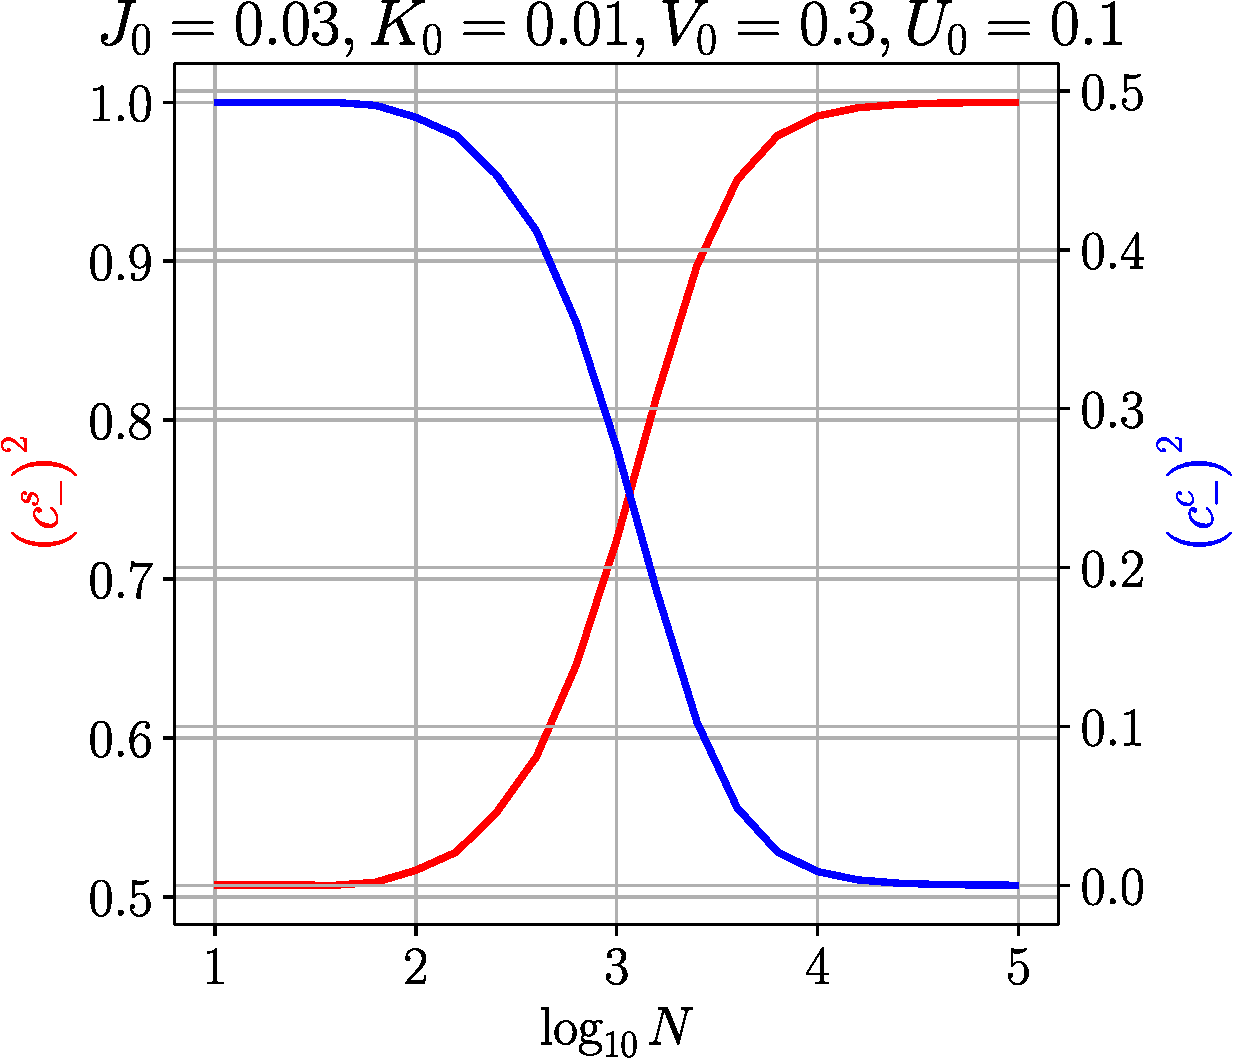
\includegraphics[width=0.52\textwidth]{../figures/cscc_q1.pdf}
	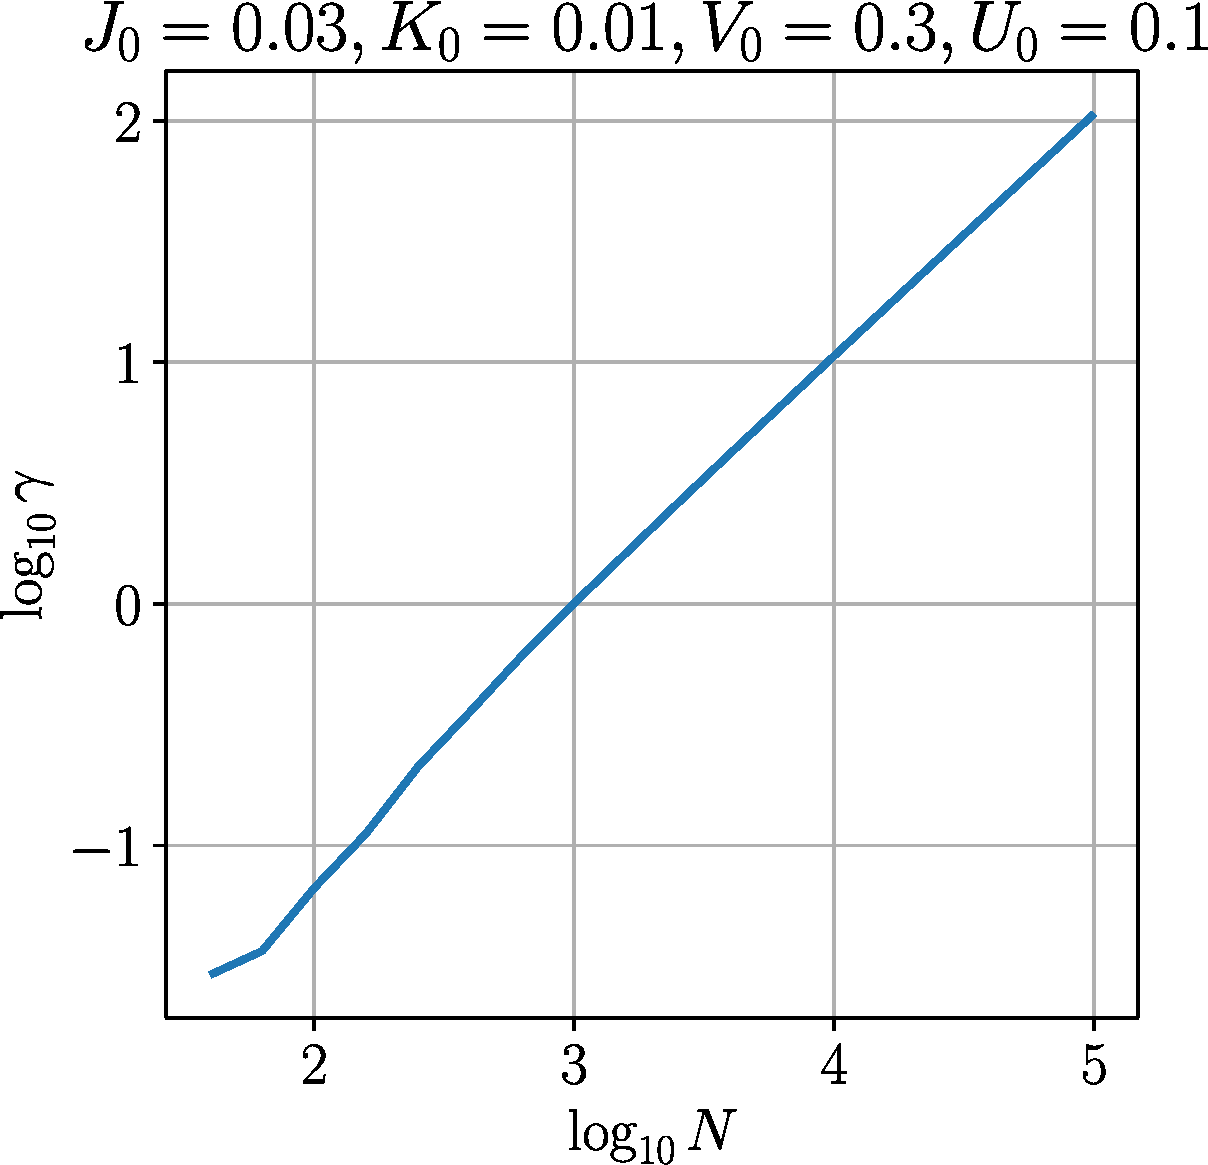
\includegraphics[width=0.46\textwidth]{../figures/gamma_q1.pdf}
	\caption{\textit{Left}: Variation of the probabilities \(\left(c^s\right)^2\) and \(\left(c^c\right)^2\) with system size. \textit{Right}: Variation of \(\gamma\) with system size.}
	\label{gamma}
\end{figure}

The full list of eigenstates is
\begin{table}[htb!]
	\centering
	\begin{tabular}{|c|c|c|c|}
		\hline
		\(\hat n\) & \(S^z\) & eigenstate & eigenvalue\\
		\hline
		0 & 0 & \(\ket{0,0}\) & \(\frac{1}{4}k\)\\
		4 & 0 & \(\ket{2,2}\) & \(\frac{1}{4}k\)\\
		\multirow{2}{*}{1} & \(\frac{1}{2}\) & \(-4v\ket{\uparrow,0} +2 \left[ \epsilon_d \mp \Delta\left(\epsilon_d , v\right)\right] \ket{0, \uparrow}\) & \multirow{4}{*}{\(\frac{1}{2} \epsilon_d \pm \frac{1}{2}\Delta\left(\epsilon_d , v\right)\)}\\
		 & - \(\frac{1}{2}\) & \(-4v\ket{\downarrow,0} +2 \left[ \epsilon_d \mp \Delta\left(\epsilon_d , v\right)\right] \ket{0, \downarrow}\)  &\\
		\multirow{2}{*}{3} & \(\frac{1}{2}\) & \(-4v\ket{\uparrow,2} +2 \left[ \epsilon_d \mp \Delta\left(\epsilon_d , v\right)\right] \ket{2, \uparrow}\) &\\
		 & - \(\frac{1}{2}\) & \(-4v\ket{\downarrow,2} +2 \left[ \epsilon_d \mp \Delta\left(\epsilon_d , v\right)\right] \ket{2, \downarrow}\)  &\\
		\multirow{5}{*}{2} & 1,-1 & \(\ket{\uparrow,\uparrow}\), \(\ket{\downarrow,\downarrow}\) & \multirow{2}{*}{\(\epsilon_d + \frac{1}{4}j\)}\\
		& \multirow{3}{*}{0} & \(\ket{\uparrow,\downarrow} + \ket{\downarrow, \uparrow}\) & \\
		& & \(\ket{2,0} - \ket{0,2}\) & \(-\frac{3}{4}k\)\\
		& & \(c_\pm^s \frac{1}{\sqrt 2}\left(\ket{\uparrow, \downarrow} - \ket{\downarrow, \uparrow}\right) + c^c_\pm \frac{1}{\sqrt 2}\left(\ket{\uparrow\downarrow, 0} + \ket{0, \uparrow\downarrow}\right)\) & \(v\left[ \gamma \pm \sqrt{\gamma^2 + 4} \right] + \epsilon_d - \frac{3}{4}j\)\\
		\hline
	\end{tabular}
	\caption{Eigenstates for effective two-site Hamiltonian}
	\label{tab:label}
\end{table}

Although \(E^2_-\) is the ground state of this two-dimensional subspace, we haven't yet checked what is the true ground state of the full Hilbert space. The eigenstates eq.~\ref{1} through \ref{2} are obviously higher than \(E_-^2\), because of the presence of the singlet \(- \frac{3}{4}j\) and the negative \(\gamma\) contribution in \(E_-^2\) compared to the positive triplet contribution \( \frac{1}{4}j\) in those equations. The only other competitors are the one in eq.~\ref{hikari} which we call \(E_c^2\), and the low energy eigenstate in eq.~\ref{low}, which we call \(E_-^1\). We first shown that \(E_-^1 > E_-^2\). The difference between \(E_-^2\) and \(E_-^1\) is
\begin{equation}\begin{aligned}
	E_-^2 - E_-^1= - \frac{3}{4}\left( j + k \right) - \sqrt{4v^2 + \frac{\epsilon_d^2}{4} + \frac{9}{64}\left( j - k \right) ^2 - \frac{3}{8}\epsilon_d\left( j-k \right) } + \sqrt{ \frac{1}{4}\epsilon_d^2 + v^2}
\end{aligned}\end{equation}
From the nature of the fixed point phases, we know that 
\begin{equation}\begin{aligned}
	J^* > K^* \implies \epsilon_d^* \leq 0
\end{aligned}\end{equation}
and
\begin{equation}\begin{aligned}
	J^* < K^* \implies \epsilon_d^* \geq 0
\end{aligned}\end{equation}
such that
\begin{equation}\begin{aligned}
	\epsilon_d\left( j-k \right) \leq 0
\end{aligned}\end{equation}
This result then very easily implies that
\begin{equation}\begin{aligned}
	4v^2 + \frac{\epsilon_d^2}{4} + \frac{9}{64}\left( j - k \right) ^2 - \frac{3}{8}\epsilon_d\left( j-k \right) > \frac{1}{4}\epsilon_d^2 + v^2
\end{aligned}\end{equation}
and we can apply this inequality to the difference between \(E_-^2\) and \(E_-^1\) to see that \(E_-^2\) is greater that \(E_-^1\).

We now compare \(E_-^2\) and \(E_c^2\):
\begin{equation}\begin{aligned}
	\Delta E_g \equiv E_-^2 - E_c^2 = \frac{1}{2}\epsilon_d - \frac{3j + k}{8} + k - \sqrt{4v^2 + \left(\frac{3j+k}{8} -\frac{1}{2} \epsilon_d\right) ^2}
\end{aligned}\end{equation}
Because of the presence of the large \(v\) in the first quadrant, this will necessarily be negative there. So, the true ground state in the first quadrant is \(E_-^2\). In the third quadrant, the large value of \(k\) will make the difference positive and the true ground state will be the charge singlet. 

These conclusions have been checked numerically and shown in fig.~\ref{fig_gstate}, where we have plotted the sign of \(\Delta E_g\) as a function of \(K_0 - J_0\). For positive values of \(K_0 - J_0\), we are in the third quadrant, and the sign of \(\Delta E_g\) being \(+1\) implies that \(E_-^2 > E_c^2\), and so the third quadrant ground state is the charge singlet (\(E_c^2\)). On the other hand, as \(K_0 - J_0\) becomes negative, we move into the first quadrant, and the sign of \(\Delta E_g\) also flips, implying that we have a transition from the charge singlet to the (mostly) spin-singlet ground state.
\begin{figure}[!htb]
	\centering
	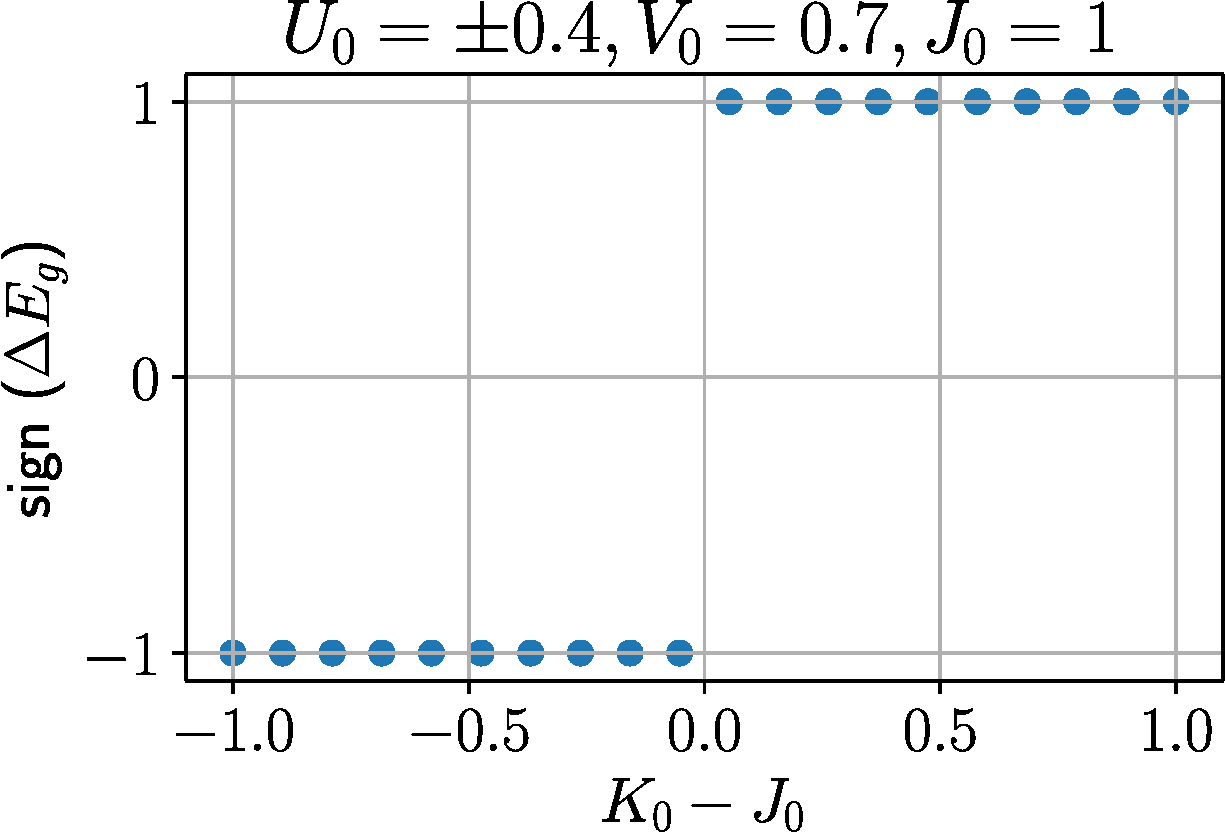
\includegraphics[width=0.5\textwidth]{../figures/gstate.pdf}
	\captionof{figure}{Shift of ground state in going from the first to third quadrant, depicted via the switch in sign of \(\Delta E_g\).}
	\label{fig_gstate}
\end{figure}

One of the most striking conclusions of this chapter is that the renormalized ground state of the SIAM in the Kondo regime is purely a singlet. The holon-doublon contributions of the ground state die out in the limit of large system size, and we are left purely with spin-sector contributions. This is, as far as we can see, due to two reasons: 
\begin{itemize}
	\item a higher RG flow rate of \(J\) as compared to \(V\)
	\item the fact that \(j \sim J N\) while \(v \sim V\sqrt N \)
\end{itemize}
These two factors help the s-d interaction term in becoming the most dominant term in the Hamiltonian, at the fixed point.

\section{Effective temperature scale at the fixed point}
We will first change the discrete RG equation to a continuum equation by interpreting \(\Delta J\) as \(\frac{\Delta J}{\Delta \ln D}\), where the denominator is unity: \(\Delta \ln D = 1\). Now, since the bandwidth is decreasing under the RG, we can write \(\Delta \ln D = -d \ln D\). The continuum equation (for \(K=0\)) becomes
\begin{equation}\begin{aligned}
	\frac{\:\mathrm{d}J}{\:\mathrm{d}\ln D} = n(0)J^2 \frac{1}{\omega - \frac{D}{2} + \frac{J}{4}}
\end{aligned}\end{equation}
where we have replaced by the number of states at each shell with that at the Fermi surface (uniform DOS). We can define a dimensionless quantity \(g \equiv \frac{J}{\frac{D}{2}} - \omega\). In terms of \(g\), the continuum RG equation becomes
\begin{equation}\begin{aligned}
	-\frac{\:\mathrm{d}g}{\:\mathrm{d}\ln D} + \frac{D g}{2\omega - D} = \frac{n(0) g^2}{1 - \frac{g}{4}}
\end{aligned}\end{equation}
Now, for the specific case where \(D\) is small (\(D \to 0\)), we can simplify and integrate this equation:
\begin{equation}\begin{aligned}
	\frac{\:\mathrm{d}g}{\:\mathrm{d}\ln D} &= \frac{n(0) g^2}{\frac{g}{4} - 1}\\
	\implies \left[\frac{1}{g} + \frac{1}{4}\ln g\right]_{g_0}^{g^*} &= n(0)\ln D\big\vert_{D_0}^{D^*}
\end{aligned}\end{equation}
\(g^*(_0), D^*(_0)\) are the fixed point (bare) values of \(g, D\). From the denominator structure, the fixed-point value is \(g^* =  4\). This gives an estimate of the bandwidth of the emergent window:
\begin{equation}\begin{aligned}
	D^* = D_0 \left( \frac{4}{g_0} \right)^\frac{1}{4n(0)}\exp\left\{-\frac{1}{n(0)}\left(\frac{1}{g_0} - \frac{1}{4}\right)\right\}
\end{aligned}\end{equation}
We can now define a temperature scale for the fixed-point theory:
\begin{equation}\begin{aligned}
	T_K \equiv \frac{2N^*}{\pi}D^* = \frac{2N^*}{\pi}D_0 \left( \frac{4}{g_0} \right)^\frac{1}{4n(0)}\exp\left\{-\frac{1}{n(0)}\left(\frac{1}{g_0} - \frac{1}{4}\right)\right\}
\end{aligned}\end{equation}
The factor of \(2N^*\) is inserted to make the Kondo temperature intensive (we will see below that the \(N^*\) allows it to  be written in terms of parameters of the two-site Hamiltonian) - \(2N^*\) is the total number of momentum states in the fixed point theory. The factor of \(\frac{1}{\pi}\) is for aesthetic reasons. Since we have and will primarily work with \(\omega=0\), the fixed point condition can be used to write \(D^* = \frac{J^* + K^*}{2}\).
\begin{equation}\begin{aligned}
	T_K = \frac{2N^*}{\pi}\frac{1}{2}\left(J^* + K^*\right) = \frac{1}{\pi}\left(j + k\right)
\end{aligned}\end{equation}
